\documentclass[12pt]{article}
%\usepackage[utf8]{inputenc}
%\documentclass[UTF8]{ctexart}
%\usepackage[UTF8, heading = false, scheme = plain]{ctex}
\usepackage{geometry}
%geometry{a4paper,scale=0.9}
\geometry{a4paper,left=1cm,right=1cm,top=1cm,bottom=2cm}
\usepackage{amsfonts}
\usepackage{color}
\usepackage{url}
%\usepackage{biblatex}
\usepackage{amsmath}
\usepackage{amssymb}
\usepackage{latexsym}
\usepackage{listings}
\usepackage[usenames,dvipsnames]{xcolor}
\usepackage{cite}
%\addbibresource{ref.bib}
%\bibliography{ref.bib}
\usepackage{caption}
\usepackage{graphicx, subfig}
\usepackage{float}
%\usepackage[fontset=ubuntu]{ctex}
%\usepackage{fontspec}
\usepackage{xeCJK}
%\usepackage[colorlinks,
%anchorcolor=black,
%citecolor=black]{hyperref}
%\setmainfont{SimSun}
\usepackage[section]{placeins}
\usepackage{enumitem}
\usepackage{framed}
\usepackage[framemethod=TikZ]{mdframed}
\usepackage{indentfirst}
\usepackage{setspace}%使用间距宏包
\linespread{1.5}
\definecolor{mygreen}{rgb}{0,0.6,0}
\definecolor{mygray}{rgb}{0.5,0.5,0.5}
\definecolor{mybgray}{rgb}{0.95,0.95,0.95}
\definecolor{mymauve}{rgb}{0.58,0,0.82}
\lstset{
 backgroundcolor=\color{mybgray}, 
 basicstyle = \footnotesize,       
 breakatwhitespace = false,        
 breaklines = true,                 
 captionpos = b,                    
 commentstyle = \color{mygreen}\bfseries,
 extendedchars = false,             
 frame =shadowbox, 
 framerule=0.5pt,
 keepspaces=true,
 keywordstyle=\color{blue}\bfseries, % keyword style
 language = C++,                     % the language of code
 otherkeywords={string}, 
 numbers=left, 
 numbersep=5pt,
 numberstyle=\tiny\color{mygray},
 rulecolor=\color{black},         
 showspaces=false,  
 showstringspaces=false, 
 showtabs=false,    
 stepnumber=1,         
 stringstyle=\color{mymauve},        % string literal style
 tabsize=2,          
 title=\lstname                      
}

\title{动态规划}
\author{leolinuxer}
%\date{June 2020}

\begin{document}
%\setlength{\parindent}{0pt}
\maketitle
\tableofcontents

\section{简单说明}
\subsection{动态规划的简单理解 \cite{Simple_DynamicProgramming}}
quora上有这样一个问题: How should I explain dynamic programming to a 4-year-old?

*writes down "1+1+1+1+1+1+1+1 =" on a sheet of paper*

"What's that equal to?"

*counting* "Eight!"

*writes down another "1+" on the left*

"What about that?"

*quickly* "Nine!"

"How'd you know it was nine so fast?"

"You just added one more"

"So you didn't need to recount because you remembered there were eight!Dynamic Programming is just a fancy way to say 'remembering stuff to save time later'"

动态规划是把大问题拆成若干个小问题;但是一个问题能否用动态规划求解的核心是:这些分拆后的小问题能不能被重复调用。

\textbf{简单理解就是:动态规划相当于递归算法,再加上记忆功能。}

\subsection{应用动态规划\cite{Simple_DynamicProgramming-2}}
如果一个问题满足以下两点,那么它就能用动态规划解决:

\begin{itemize}[itemindent=2em]
    \item 问题的答案依赖于问题的规模,也就是问题的所有答案构成了一个数列:$\{f(1),f(2), \cdots, f(n)\}$,其中 $n$ 是问题的规模。
    
    \item 大规模问题的答案可以由小规模问题的答案递推得到,也就是说 $f(n)$ 的值可以由 $\{f(i)|i<n\}$ 中的个别求得。
\end{itemize}

那么如何应用动态规划呢?可以将动态规划拆分成三个子目标:

\begin{enumerate}[itemindent=2em]
    \item 建立状态转移方程。当做已经知道的值$\{f(1),f(2), \cdots, f(n-1)\}$,然后想办法利用它们求得$f(n)$。
    
    \item 缓存并复用以往结果。这一步不难,但是很重要。如果没有合适地处理,很有可能就是指数和线性时间复杂度的区别。

    \item 按顺序从小往大算。这里的“小”和“大”对应的是问题的规模,在这里也就是我们要从 $f(1), f(2), \cdots, $ 到 $f(n)$ 依次顺序计算。
\end{enumerate}

\section{动态规划详解\cite{F_Algorithm_Dynamic_Programming_Step}}
\subsection{概述}
\textbf{动态规划问题的一般形式就是求最值}。动态规划其实是运筹学的一种最优化方法,只不过在计算机问题上应用比较多,比如说让你求最长递增子序列呀,最小编辑距离呀等等。既然是要求最值,核心问题是什么呢?\textbf{求解动态规划的核心问题是穷举}。因为要求最值,肯定要把所有可行的答案穷举出来,然后在其中找最值呗。

动态规划就这么简单,就是穷举就完事了?我看到的动态规划问题都很难啊!

首先,动态规划的穷举有点特别,因为这类问题存在\textbf{「重叠子问题」},如果暴力穷举的话效率会极其低下,所以需要「备忘录」或者「DP table」来优化穷举过程,避免不必要的计算。

而且,动态规划问题一定会具备\textbf{「最优子结构」},才能通过子问题的最值得到原问题的最值。

另外,虽然动态规划的核心思想就是穷举求最值,但是问题可以千变万化,穷举所有可行解其实并不是一件容易的事,只有\textbf{列出正确的「状态转移方程」}才能正确地穷举。

以上提到的\textbf{重叠子问题、最优子结构、状态转移方程就是动态规划三要素}。具体什么意思等会会举例详解,但是在实际的算法问题中,\textbf{写出状态转移方程是最困难的},这也就是为什么很多朋友觉得动态规划问题困难的原因,我来提供我研究出来的一个思维框架,辅助你思考状态转移方程:

\textbf{明确「状态」 -> 定义 dp 数组/函数的含义 -> 明确「选择」-> 明确 base case}。

下面通过斐波那契数列问题和凑零钱问题来详解动态规划的基本原理。前者主要是让你明白什么是重叠子问题(斐波那契数列严格来说不是动态规划问题),后者主要举集中于如何列出状态转移方程。

\subsection{通过斐波那契数列理解重叠子问题}
\subsubsection{暴力递归}
斐波那契数列的数学形式就是递归的,写成代码就是这样:
\begin{lstlisting}
int fib(int N) {
    if (N == 1 || N == 2) return 1;
    return fib(N - 1) + fib(N - 2);
}
}
\end{lstlisting}

我们知道这样写代码虽然简洁易懂,但是十分低效,低效在哪里?假设 n = 20,请画出递归树。\textbf{PS:但凡遇到需要递归的问题,最好都画出递归树,这对你分析算法的复杂度,寻找算法低效的原因都有巨大帮助。}
\begin{figure}[H]
    \centering
    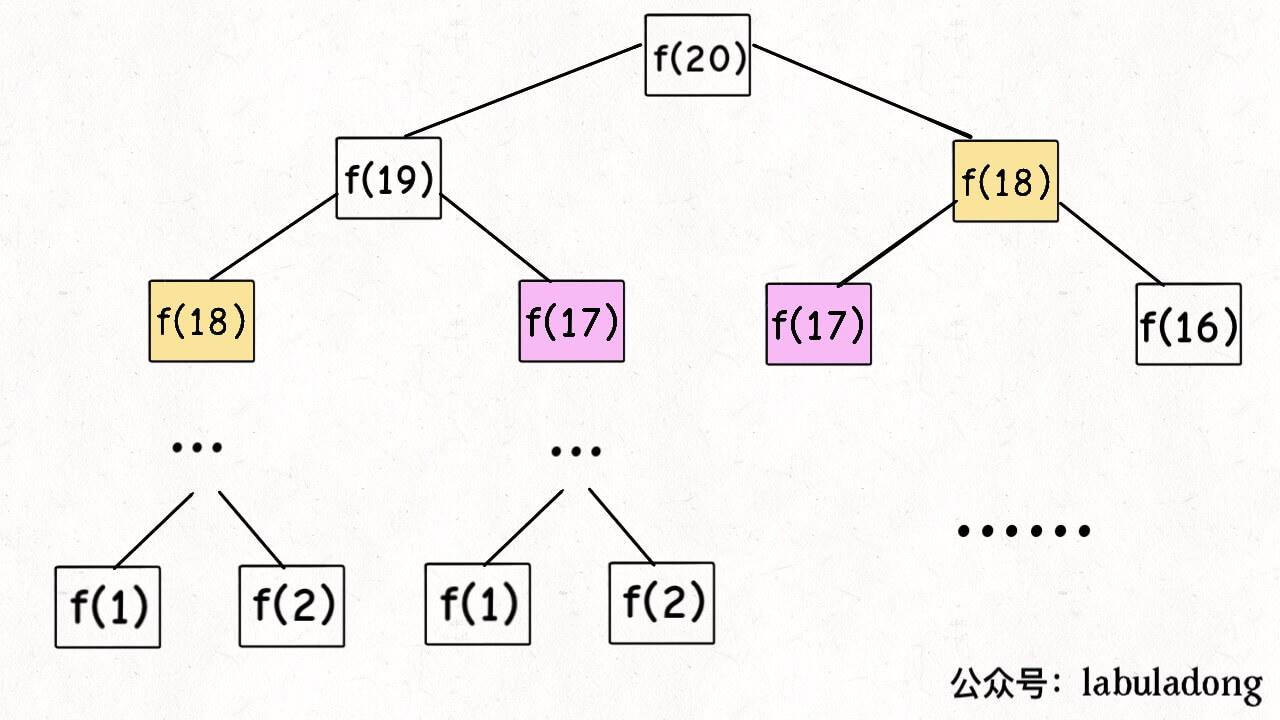
\includegraphics[width=.5\textwidth]{fig/Dynamic_Programming_Recursion_Tree_1.jpg}
\end{figure}

这个递归树怎么理解?就是说想要计算原问题 f(20),我就得先计算出子问题 f(19) 和 f(18),然后要计算 f(19),我就要先算出子问题 f(18) 和 f(17),以此类推。最后遇到 f(1) 或者 f(2) 的时候,结果已知,就能直接返回结果,递归树不再向下生长了。

\textbf{递归算法的时间复杂度怎么计算?子问题个数乘以解决一个子问题需要的时间。}

子问题个数,即递归树中节点的总数。显然二叉树节点总数为指数级别,所以子问题个数为 $O(2^n)$;解决一个子问题的时间,在本算法中,没有循环,只有 f(n - 1) + f(n - 2) 一个加法操作,时间为 O(1)。所以,这个算法的时间复杂度为  $O(2^n)$,指数级别,爆炸。

观察递归树,很明显发现了算法低效的原因:存在大量重复计算,比如 f(18) 被计算了两次,而且你可以看到,以 f(18) 为根的这个递归树体量巨大,多算一遍,会耗费巨大的时间。更何况,还不止 f(18) 这一个节点被重复计算,所以这个算法及其低效。

\subsubsection{带备忘录的递归解法}
明确了问题,其实就已经把问题解决了一半。即然耗时的原因是重复计算,那么我们可以造一个「备忘录」,每次算出某个子问题的答案后别急着返回,先记到「备忘录」里再返回;每次遇到一个子问题先去「备忘录」里查一查,如果发现之前已经解决过这个问题了,直接把答案拿出来用,不要再耗时去计算了。一般使用一个数组充当这个「备忘录」,当然你也可以使用哈希表(字典),思想都是一样的。
\begin{lstlisting}
int fib(int N) {
    if (N < 1) return 0;
    vector<int> memo(N + 1, 0);     // 备忘录全初始化为 0
    return helper(memo, N); 	    // 初始化最简情况
}
 
int helper(vector<int>& memo, int n) {
    // base case 
    if (n == 1 || n == 2) return 1;
    if (memo[n] != 0) return memo[n];     // 已经计算过
    memo[n] = helper(memo, n - 1) + helper(memo, n - 2);
    return memo[n];
}
\end{lstlisting}
现在,画出递归树,你就知道「备忘录」到底做了什么。
\begin{figure}[H]
    \centering
    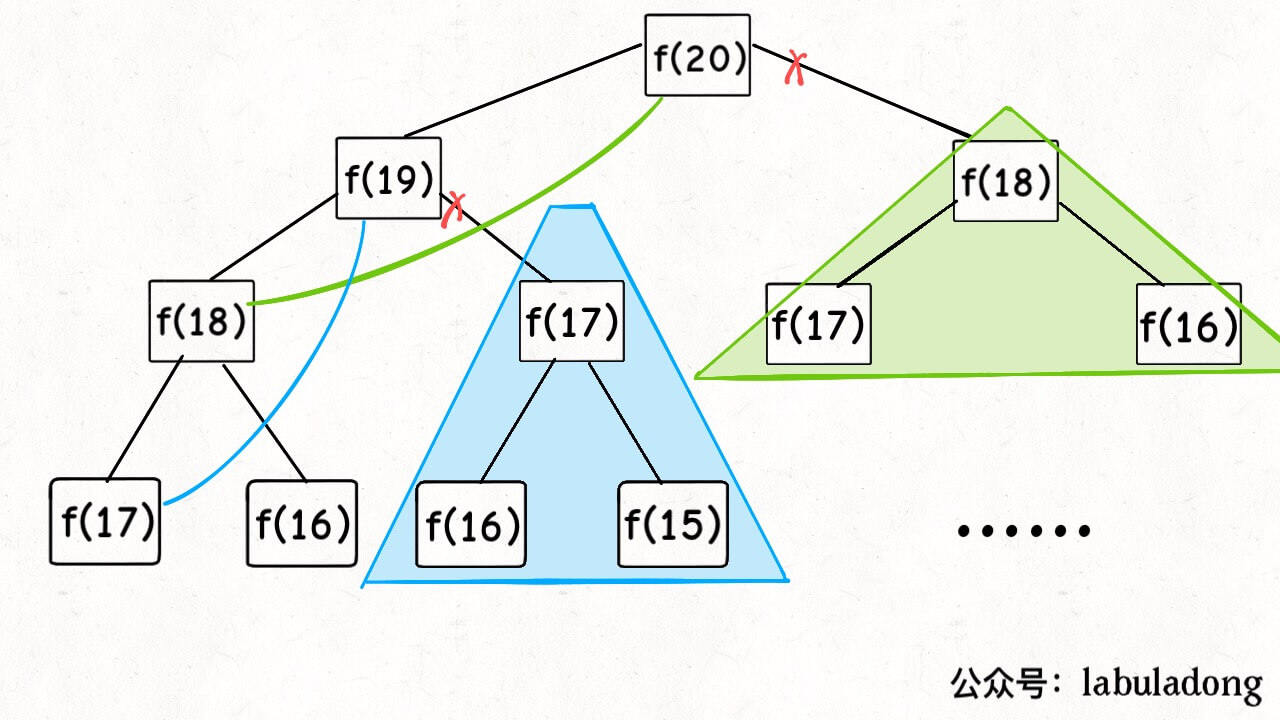
\includegraphics[width=.5\textwidth]{fig/Dynamic_Programming_Recursion_Tree_2.jpg}
\end{figure}

实际上,带「备忘录」的递归算法,把一棵存在巨量冗余的递归树通过「剪枝」,改造成了一幅不存在冗余的递归图,极大减少了子问题(即递归图中节点)的个数。
\begin{figure}[H]
    \centering
    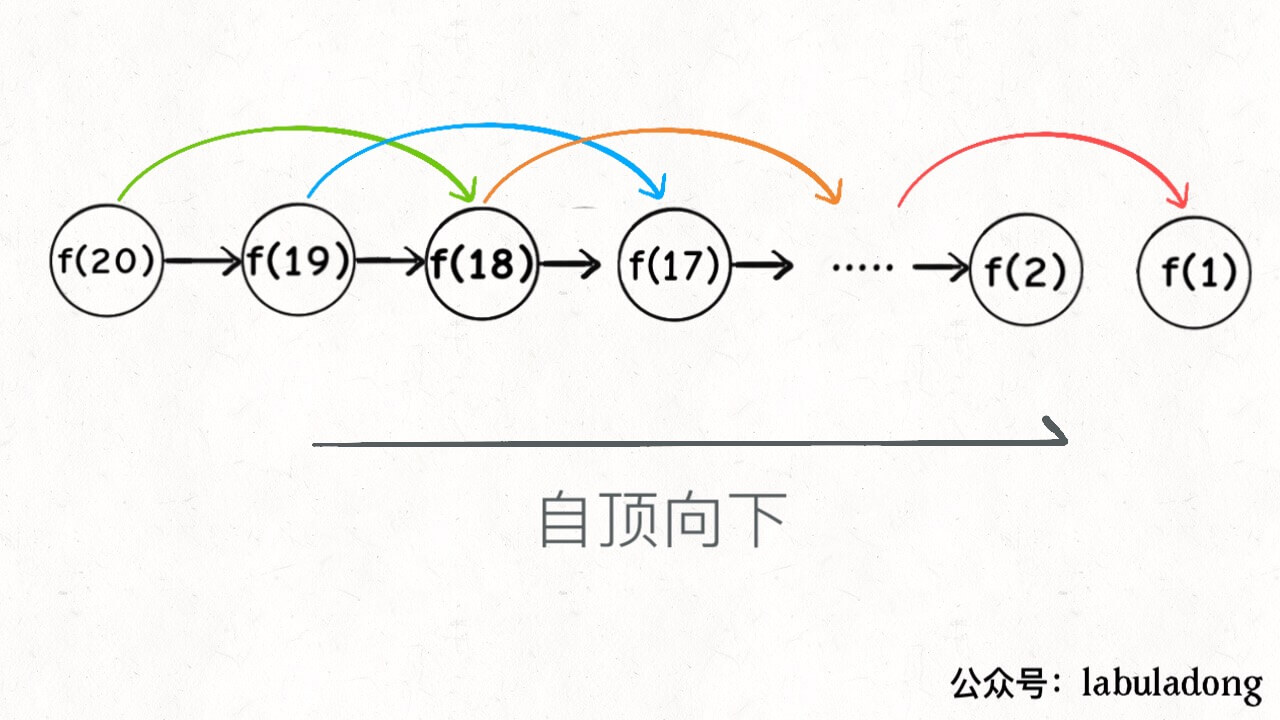
\includegraphics[width=.5\textwidth]{fig/Dynamic_Programming_Recursion_Tree_3.jpg}
\end{figure}

递归算法的时间复杂度怎么算?子问题个数乘以解决一个子问题需要的时间。子问题个数,即图中节点的总数,由于本算法不存在冗余计算,子问题就是 f(1), f(2), f(3) ... f(20),数量和输入规模 n = 20 成正比,所以子问题个数为 O(n)。解决一个子问题的时间,同上,没有什么循环,时间为 O(1)。所以,本算法的时间复杂度是 O(n)。比起暴力算法,是降维打击。

至此,带备忘录的递归解法的效率已经和迭代的动态规划解法一样了。实际上,这种解法和迭代的动态规划已经差不多了,\textbf{只不过这种方法叫做「自顶向下」,动态规划叫做「自底向上」}。

啥叫「自顶向下」?注意我们刚才画的递归树(或者说图),是从上向下延伸,都是从一个规模较大的原问题比如说 f(20),向下逐渐分解规模,直到 f(1) 和 f(2) 触底,然后逐层返回答案,这就叫「自顶向下」。

啥叫「自底向上」?反过来,我们直接从最底下,最简单,问题规模最小的 f(1) 和 f(2) 开始往上推,直到推到我们想要的答案 f(20),这就是动态规划的思路,这也是为什么\textbf{动态规划一般都脱离了递归,而是由循环迭代完成计算}。

\subsubsection{dp 数组的迭代解法}
有了上一步「备忘录」的启发,我们可以把这个「备忘录」独立出来成为一张表,就叫做 DP table 吧,在这张表上完成「自底向上」的推算岂不美哉!
\begin{lstlisting}
int fib(int N) {
    vector<int> dp(N + 1, 0);
    // base case
    dp[1] = dp[2] = 1;
    for (int i = 3; i <= N; i++)
        dp[i] = dp[i - 1] + dp[i - 2];
    return dp[N];
}
\end{lstlisting}
\begin{figure}[H]
    \centering
    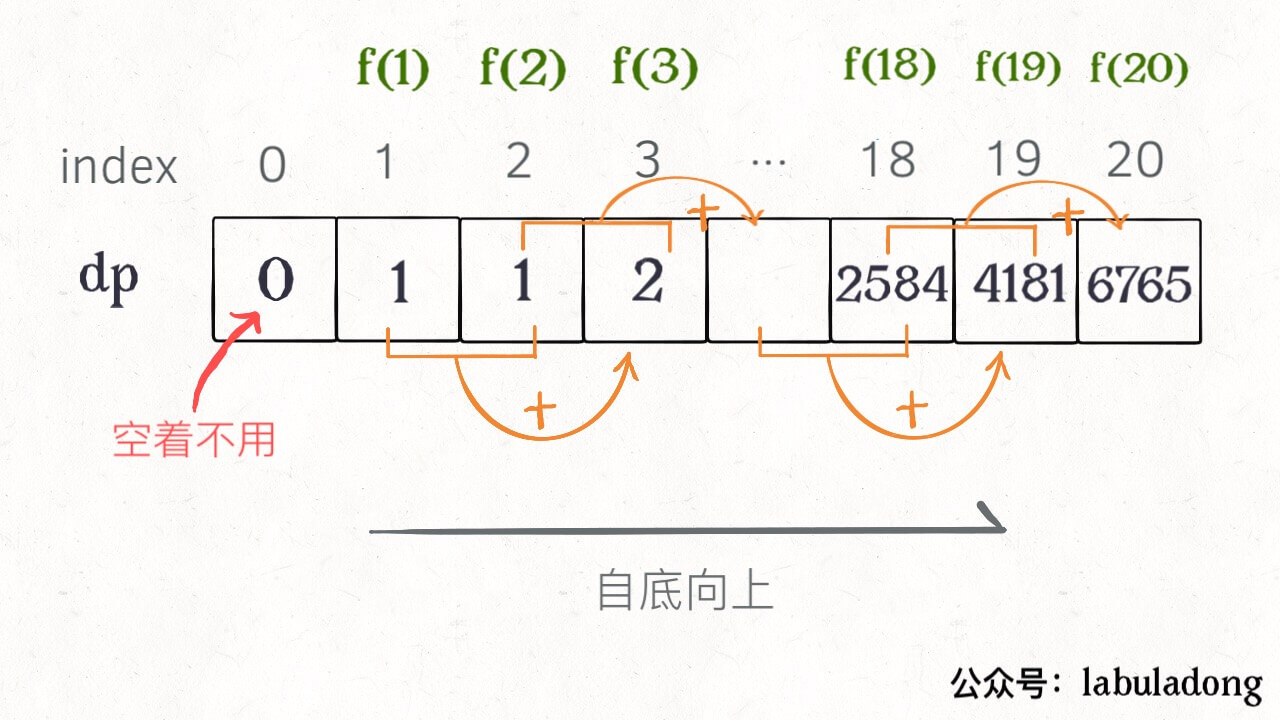
\includegraphics[width=.5\textwidth]{fig/Dynamic_Programming_Recursion_Tree_4.jpg}
\end{figure}

画个图就很好理解了,而且你发现这个 DP table 特别像之前那个「剪枝」后的结果,只是反过来算而已。实际上,带备忘录的递归解法中的「备忘录」,最终完成后就是这个 DP table,所以说这两种解法其实是差不多的,大部分情况下,效率也基本相同。

这里,引出「状态转移方程」这个名词,实际上就是描述问题结构的数学形式。
\begin{figure}[H]
    \centering
    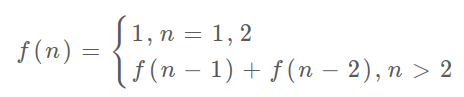
\includegraphics[width=.5\textwidth]{fig/Dynamic_Programming_Status_Transition.png}
\end{figure}

为啥叫「状态转移方程」?为了听起来高端。你把 f(n) 想做一个状态 n,这个状态 n 是由状态 n - 1 和状态 n - 2 相加转移而来,这就叫状态转移,仅此而已。你会发现,上面的几种解法中的所有操作,例如 return f(n - 1) + f(n - 2),dp[i] = dp[i - 1] + dp[i - 2],以及对备忘录或 DP table 的初始化操作,都是围绕这个方程式的不同表现形式。可见列出「状态转移方程」的重要性,它是解决问题的核心。很容易发现,其实状态转移方程直接代表着暴力解法。

千万不要看不起暴力解,动态规划问题最困难的就是写出状态转移方程,即这个暴力解。优化方法无非是用备忘录或者 DP table,再无奥妙可言。

这个例子的最后,讲一个细节优化。细心的读者会发现,根据斐波那契数列的状态转移方程,当前状态只和之前的两个状态有关,其实并不需要那么长的一个 DP table 来存储所有的状态,只要想办法存储之前的两个状态就行了。所以,可以进一步优化,把空间复杂度降为 O(1):
\begin{lstlisting}
int fib(int n) {
    if (n == 2 || n == 1) 
        return 1;
    int prev = 1, curr = 1;
    for (int i = 3; i <= n; i++) {
        int sum = prev + curr;
        prev = curr;
        curr = sum;
    }
    return curr;
}
\end{lstlisting}

有人会问,动态规划的另一个重要特性「最优子结构」,怎么没有涉及?下面会涉及。斐波那契数列的例子严格来说不算动态规划,因为没有涉及求最值,以上旨在演示算法设计螺旋上升的过程。下面,看第二个例子,凑零钱问题。

\subsection{通过凑零钱问题理解最优子结构}
先看下题目:给你 k 种面值的硬币,面值分别为 c1, c2 ... ck,每种硬币的数量无限,再给一个总金额 amount,问你最少需要几枚硬币凑出这个金额,如果不可能凑出,算法返回 -1 。算法的函数签名如下:
\begin{lstlisting}
// coins 中是可选硬币面值,amount 是目标金额
int coinChange(int[] coins, int amount);
\end{lstlisting}

比如说 k = 3,面值分别为 1,2,5,总金额 amount = 11。那么最少需要 3 枚硬币凑出,即 11 = 5 + 5 + 1。

你认为计算机应该如何解决这个问题?显然,就是把所有可能的凑硬币方法都穷举出来,然后找找看最少需要多少枚硬币。

\subsubsection{暴力递归}
首先,这个问题是动态规划问题,因为它具有「最优子结构」的。\textbf{要符合「最优子结构」,子问题间必须互相独立}。啥叫相互独立?你肯定不想看数学证明,我用一个直观的例子来讲解。

比如说,你的原问题是考出最高的总成绩,那么你的子问题就是要把语文考到最高,数学考到最高…… 为了每门课考到最高,你要把每门课相应的选择题分数拿到最高,填空题分数拿到最高…… 当然,最终就是你每门课都是满分,这就是最高的总成绩。得到了正确的结果:最高的总成绩就是总分。因为这个过程符合最优子结构,“每门科目考到最高”这些\textbf{子问题是互相独立,互不干扰的}。

但是,如果加一个条件:你的语文成绩和数学成绩会互相制约,此消彼长。这样的话,显然你能考到的最高总成绩就达不到总分了,按刚才那个思路就会得到错误的结果。因为子问题并不独立,语文数学成绩无法同时最优,所以最优子结构被破坏。

回到凑零钱问题,为什么说它符合最优子结构呢?比如你想求 amount = 11 时的最少硬币数(原问题),如果你知道凑出 amount = 10 的最少硬币数(子问题),你只需要把子问题的答案加一(再选一枚面值为 1 的硬币)就是原问题的答案,因为硬币的数量是没有限制的,子问题之间没有相互制,是互相独立的。

那么,既然知道了这是个动态规划问题,就要思考\textbf{如何列出正确的状态转移方程}?

\begin{itemize}
\setlength{\itemsep}{0pt}
\setlength{\parsep}{0pt}
\setlength{\parskip}{0pt}
    \item \textbf{先确定「状态」},也就是原问题和子问题中变化的变量。由于硬币数量无限,所以唯一的状态就是目标金额 amount。
    \item \textbf{然后确定 dp 函数的定义}:当前的目标金额是 n,至少需要 dp(n) 个硬币凑出该金额。
    \item \textbf{然后确定「选择」并择优},也就是对于每个状态,可以做出什么选择改变当前状态。具体到这个问题,无论当的目标金额是多少,选择就是从面额列表 coins 中选择一个硬币,然后目标金额就会减少:
    \begin{lstlisting}
# 伪码框架
def coinChange(coins: List[int], amount: int):
    # 定义:要凑出金额 n,至少要 dp(n) 个硬币
    def dp(n):
        # 做选择,选择需要硬币最少的那个结果
        for coin in coins:
            res = min(res, 1 + dp(n - coin))
        return res
    # 我们要求的问题是 dp(amount)
    return dp(amount)
\end{lstlisting}
   \item \textbf{最后明确 base case},显然目标金额为 0 时,所需硬币数量为 0;当目标金额小于 0 时,无解,返回 -1:
       \begin{lstlisting}
def coinChange(coins: List[int], amount: int):
    def dp(n):
        # base case
        if n == 0: return 0
        if n < 0: return -1
        # 求最小值,所以初始化为正无穷
        res = float('INF')
        for coin in coins:
            subproblem = dp(n - coin)
            # 子问题无解,跳过
            if subproblem == -1: continue
            res = min(res, 1 + subproblem)

        return res if res != float('INF') else -1
    
    return dp(amount)
\end{lstlisting}
\end{itemize}

至此,状态转移方程其实已经完成了,以上算法已经是暴力解法了,以上代码的数学形式就是状态转移方程:
\begin{figure}[H]
    \centering
    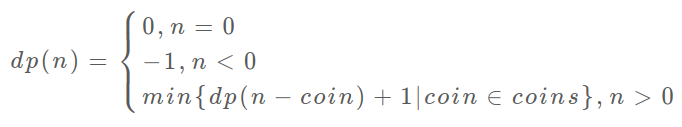
\includegraphics[width=.5\textwidth]{fig/Dynamic_Programming_Status_Transition_Coin.png}
\end{figure}

至此,这个问题其实就解决了,只不过需要消除一下重叠子问题,比如 amount = 11, coins = {1,2,5} 时画出递归树看看:
\begin{figure}[H]
    \centering
    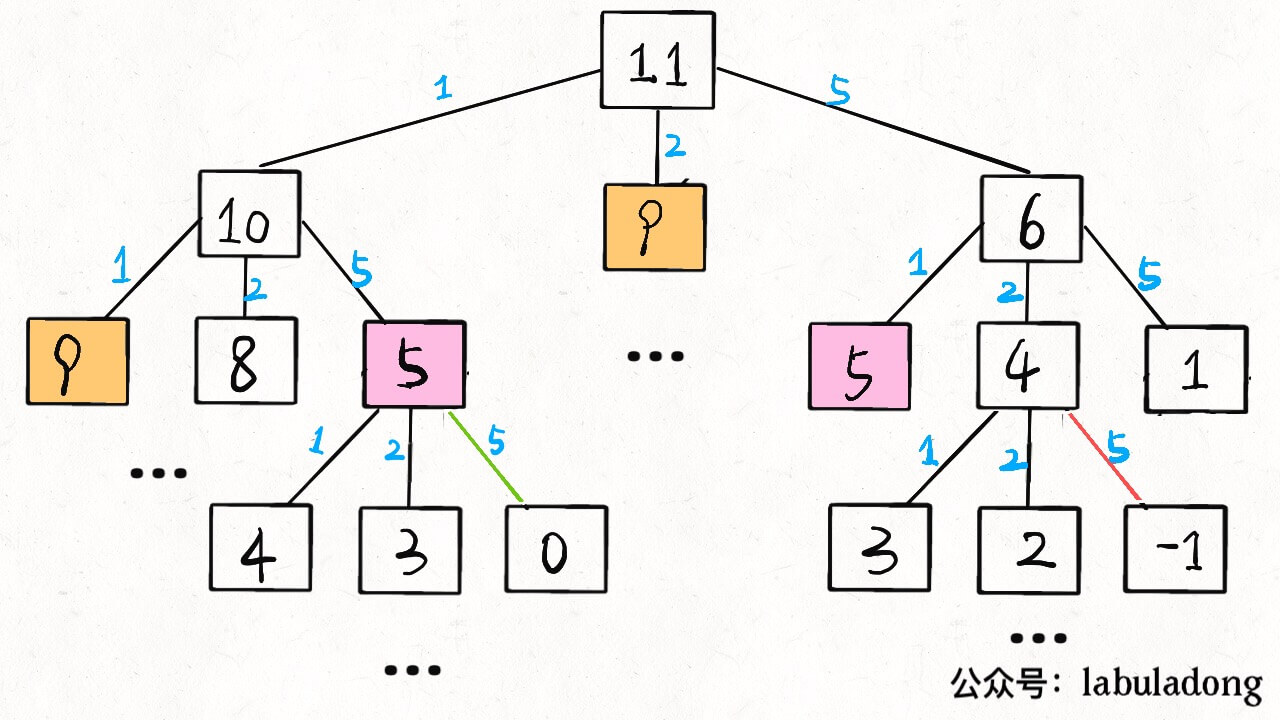
\includegraphics[width=.5\textwidth]{fig/Dynamic_Programming_Recursion_Tree_5.jpg}
\end{figure}

\textbf{时间复杂度分析:子问题总数 x 每个子问题的时间。}子问题总数为递归树节点个数,这个比较难看出来,是 $O(n^k)$,总之是指数级别的。每个子问题中含有一个 for 循环,复杂度为 $O(k)$。所以总时间复杂度为 $O(k * n^k)$,指数级别。

\subsubsection{带备忘录的递归}
只需要稍加修改,就可以通过备忘录消除子问题:
\begin{lstlisting}
def coinChange(coins: List[int], amount: int):
    # 备忘录
    memo = dict()
    def dp(n):
        # 查备忘录,避免重复计算
        if n in memo: return memo[n]

        if n == 0: return 0
        if n < 0: return -1
        res = float('INF')
        for coin in coins:
            subproblem = dp(n - coin)
            if subproblem == -1: continue
            res = min(res, 1 + subproblem)
        
        # 记入备忘录
        memo[n] = res if res != float('INF') else -1
        return memo[n]
    
    return dp(amount)
\end{lstlisting}
不画图了,很显然「备忘录」大大减小了子问题数目,完全消除了子问题的冗余,所以子问题总数不会超过金额数 n,即子问题数目为 O(n)。处理一个子问题的时间不变,仍是 O(k),所以总的时间复杂度是 O(kn)。

\subsubsection{dp 数组的迭代解法}
当然,我们也可以自底向上使用 dp table 来消除重叠子问题,dp 数组的定义和刚才 dp 函数类似,定义也是一样的:

dp[i] = x 表示,当目标金额为 i 时,至少需要 x 枚硬币。
\begin{lstlisting}
int coinChange(vector<int>& coins, int amount) {
    // 数组大小为 amount + 1,初始值也为 amount + 1
    vector<int> dp(amount + 1, amount + 1);
    // base case
    dp[0] = 0;
    for (int i = 0; i < dp.size(); i++) {
        // 内层 for 在求所有子问题 + 1 的最小值
        for (int coin : coins) {
            // 子问题无解,跳过
            if (i - coin < 0) continue;
            dp[i] = min(dp[i], 1 + dp[i - coin]);
        }
    }
    return (dp[amount] == amount + 1) ? -1 : dp[amount];
}
\end{lstlisting}

\begin{figure}[H]
    \centering
    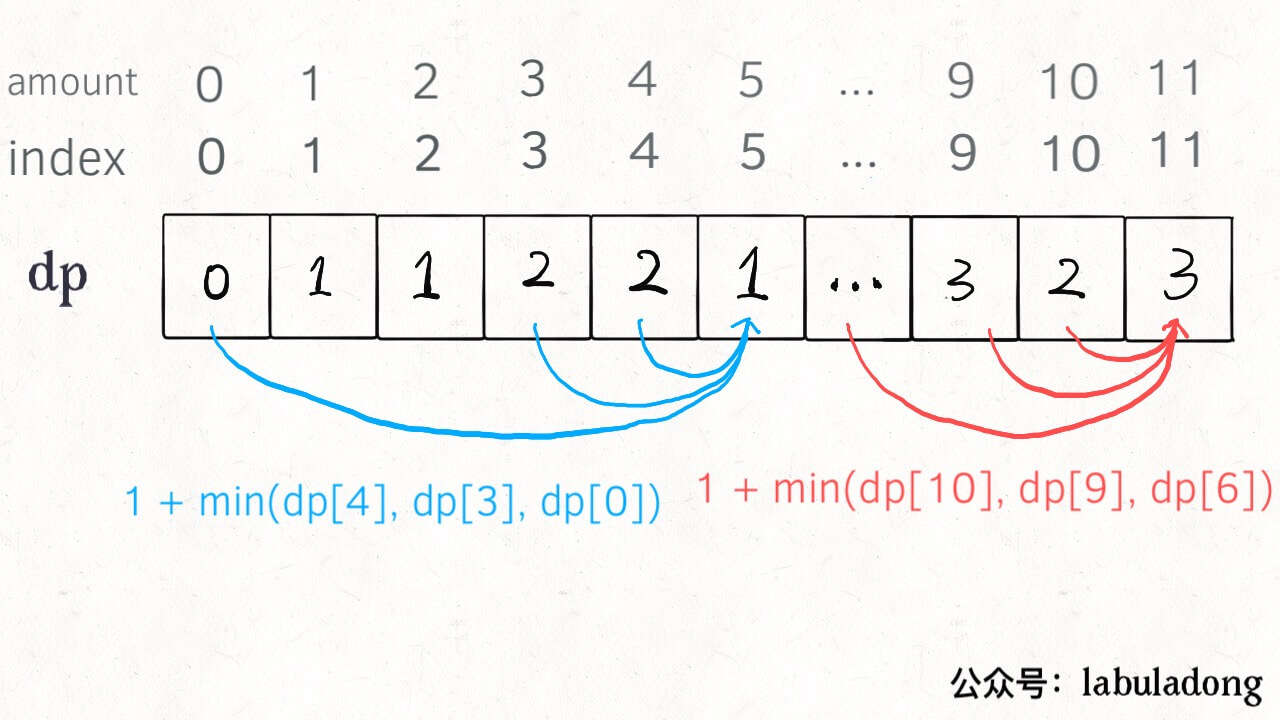
\includegraphics[width=.5\textwidth]{fig/Dynamic_Programming_Recursion_Tree_6.jpg}
\end{figure}

PS:为啥 dp 数组初始化为 amount + 1 呢,因为凑成 amount 金额的硬币数最多只可能等于 amount(全用 1 元面值的硬币),所以初始化为 amount + 1 就相当于初始化为正无穷,便于后续取最小值。

\subsection{最优子结构详解}
\url{https://github.com/labuladong/fucking-algorithm/blob/master/%E5%8A%A8%E6%80%81%E8%A7%84%E5%88%92%E7%B3%BB%E5%88%97/%E6%9C%80%E4%BC%98%E5%AD%90%E7%BB%93%E6%9E%84.md}

「最优子结构」是某些问题的一种特定性质,并不是动态规划问题专有的。也就是说,很多问题其实都具有最优子结构,只是其中大部分不具有重叠子问题,所以我们不把它们归为动态规划系列问题而已。

我先举个很容易理解的例子:假设你们学校有 10 个班,你已经计算出了每个班的最高考试成绩。那么现在我要求你计算全校最高的成绩,你会不会算?当然会,而且你不用重新遍历全校学生的分数进行比较,而是只要在这 10 个最高成绩中取最大的就是全校的最高成绩。这个问题就符合最优子结构:可以从子问题的最优结果推出更大规模问题的最优结果。让你算每个班的最优成绩就是子问题,你知道所有子问题的答案后,就可以借此推出全校学生的最优成绩这个规模更大的问题的答案。

你看,这么简单的问题都有最优子结构性质,只是因为显然没有重叠子问题,所以我们简单地求最值肯定用不出动态规划。

举个例子:假设你们学校有 10 个班,你已知每个班的最大分数差(最高分和最低分的差值)。那么现在我让你计算全校学生中的最大分数差,你会不会算?可以想办法算,但是肯定不能通过已知的这 10 个班的最大分数差推到出来。因为这 10 个班的最大分数差不一定就包含全校学生的最大分数差,比如全校的最大分数差可能是 3 班的最高分和 6 班的最低分之差。这个问题就不符合最优子结构,因为你没办通过每个班的最优值推出全校的最优值,没办法通过子问题的最优值推出规模更大的问题的最优值。前文「动态规划详解」说过,想满足最优子结,子问题之间必须互相独立。全校的最大分数差可能出现在两个班之间,显然子问题不独立,所以这个问题本身不符合最优子结构。

那么遇到这种最优子结构失效情况,怎么办?\textbf{策略是:改造问题}。对于最大分数差这个问题,我们不是没办法利用已知的每个班的分数差吗,那我只能这样写一段暴力代码:
\begin{lstlisting}
int result = 0;
for (Student a : school) {
    for (Student b : school) {
        if (a is b) continue;
        result = max(result, |a.score - b.score|);
    }
}
return result;
\end{lstlisting}
改造问题,也就是把问题等价转化:最大分数差,不就等价于最高分数和最低分数的差么,那不就是要求最高和最低分数么,不就是我们讨论的第一个问题么,不就具有最优子结构了么?那现在改变思路,借助最优子结构解决最值问题,再回过头解决最大分数差问题,是不是就高效多了?

当然,上面这个例子太简单了,不过请读者回顾一下,我们做动态规划问题,是不是一直在求各种最值,本质跟我们举的例子没啥区别,无非需要处理一下重叠子问题。

再举个常见但也十分简单的例子,求一棵二叉树的最大值,不难吧(简单起见,假设节点中的值都是非负数):
\begin{lstlisting}
int maxVal(TreeNode root) {
    if (root == null)
        return -1;
    int left = maxVal(root.left);
    int right = maxVal(root.right);
    return max(root.val, left, right);
}
\end{lstlisting}
你看这个问题也符合最优子结构,以 root 为根的树的最大值,可以通过两边子树(子问题)的最大值推导出来,结合刚才学校和班级的例子,很容易理解吧。

当然这也不是动态规划问题,旨在说明,\textbf{最优子结构并不是动态规划独有的一种性质,能求最值的问题大部分都具有这个性质};但反过来,\textbf{最优子结构性质作为动态规划问题的必要条件},一定是让你求最值的,以后碰到那种恶心人的最值题,思路往动态规划想就对了,这就是套路。

动态规划不就是从最简单的 base case 往后推导吗,可以想象成一个链式反应,以小博大。但只有符合最优子结构的问题,才有发生这种链式反应的性质。

找最优子结构的过程,其实就是证明状态转移方程正确性的过程,方程符合最优子结构就可以写暴力解了,写出暴力解就可以看出有没有重叠子问题了,有则优化,无则 OK。这也是套路,经常刷题的朋友应该能体会

\subsection{dp 数组的遍历方向}
我相信读者做动态规问题时,肯定会对 dp 数组的遍历顺序有些头疼。我们拿二维 dp 数组来举例,有时候我们是正向遍历:
\begin{lstlisting}
int[][] dp = new int[m][n];
for (int i = 0; i < m; i++)
    for (int j = 0; j < n; j++)
        // 计算 dp[i][j]
\end{lstlisting}

有时候我们反向遍历:
\begin{lstlisting}
for (int i = m - 1; i >= 0; i--)
    for (int j = n - 1; j >= 0; j--)
        // 计算 dp[i][j]
\end{lstlisting}

有时候可能会斜向遍历:
\begin{lstlisting}
// 斜着遍历数组
for (int l = 2; l <= n; l++) {
    for (int i = 0; i <= n - l; i++) {
        int j = l + i - 1;
        // 计算 dp[i][j]
    }
}
\end{lstlisting}

那么,如果仔细观察的话可以发现其中的原因的。你只要把住两点就行了:
\begin{itemize}
\setlength{\itemsep}{0pt}
\setlength{\parsep}{0pt}
\setlength{\parskip}{0pt}
    \item \textbf{遍历的过程中,所需的状态必须是已经计算出来的};
    \item \textbf{遍历的终点必须是存储结果的那个位置};
\end{itemize}

下面来具体解释上面两个原则是什么意思。

比如编辑距离这个经典的问题,我们通过对 dp 数组的定义,确定了 base case 是 dp[..][0] 和 dp[0][..],最终答案是 dp[m][n];而且我们通过状态转移方程知道 dp[i][j] 需要从 dp[i-1][j], dp[i][j-1], dp[i-1][j-1] 转移而来,如下图:
\begin{figure}[H]
    \centering
    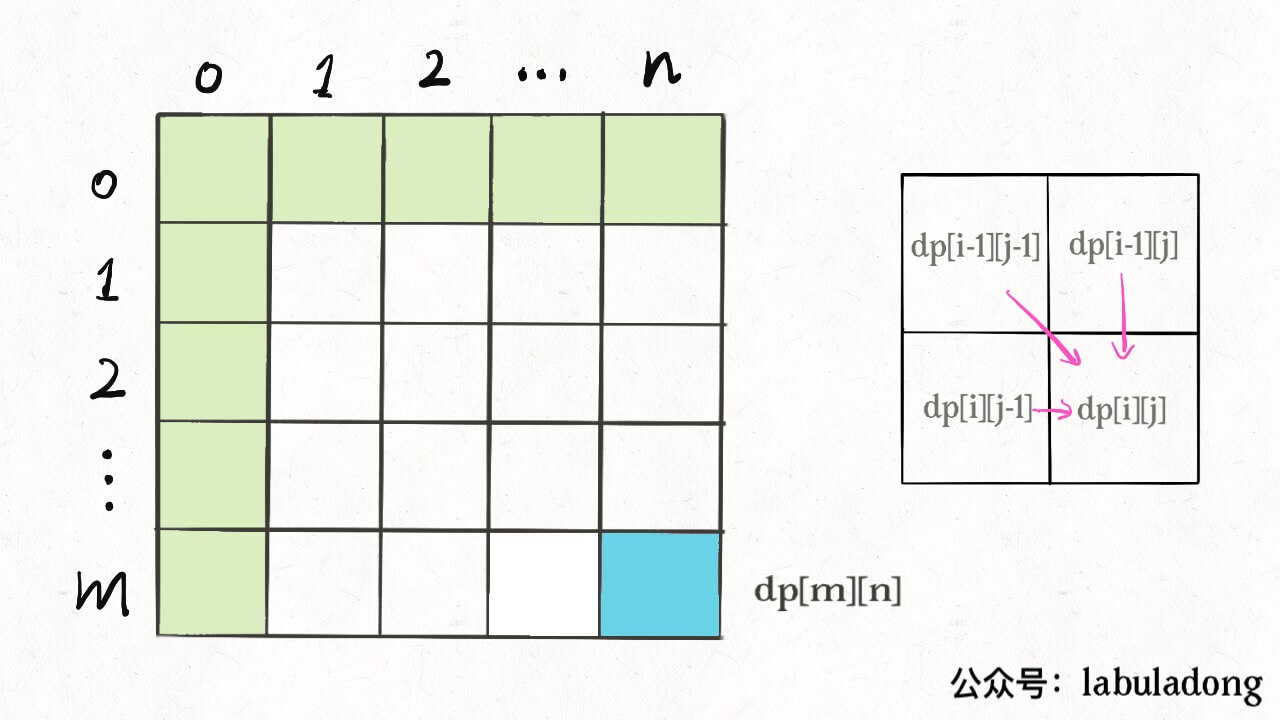
\includegraphics[width=1\textwidth]{fig/Dynamic_Programming_Optimal_Substructure_1.jpg}
\end{figure}

那么,参考刚才说的两条原则,你该怎么遍历 dp 数组?肯定是正向遍历:
\begin{lstlisting}
for (int i = 1; i < m; i++)
    for (int j = 1; j < n; j++)
        // 通过 dp[i-1][j], dp[i][j - 1], dp[i-1][j-1]
        // 计算 dp[i][j]
\end{lstlisting}
因为,这样每一步迭代的左边、上边、左上边的位置都是 base case 或者之前计算过的,而且最终结束在我们想要的答案 dp[m][n]。

再举一例,回文子序列问题,我们通过过对 dp 数组的定义,确定了 base case 处在中间的对角线,dp[i][j] 需要从 dp[i+1][j], dp[i][j-1], dp[i+1][j-1] 转移而来,想要求的最终答案是 dp[0][n-1],如下图:
\begin{figure}[H]
    \centering
    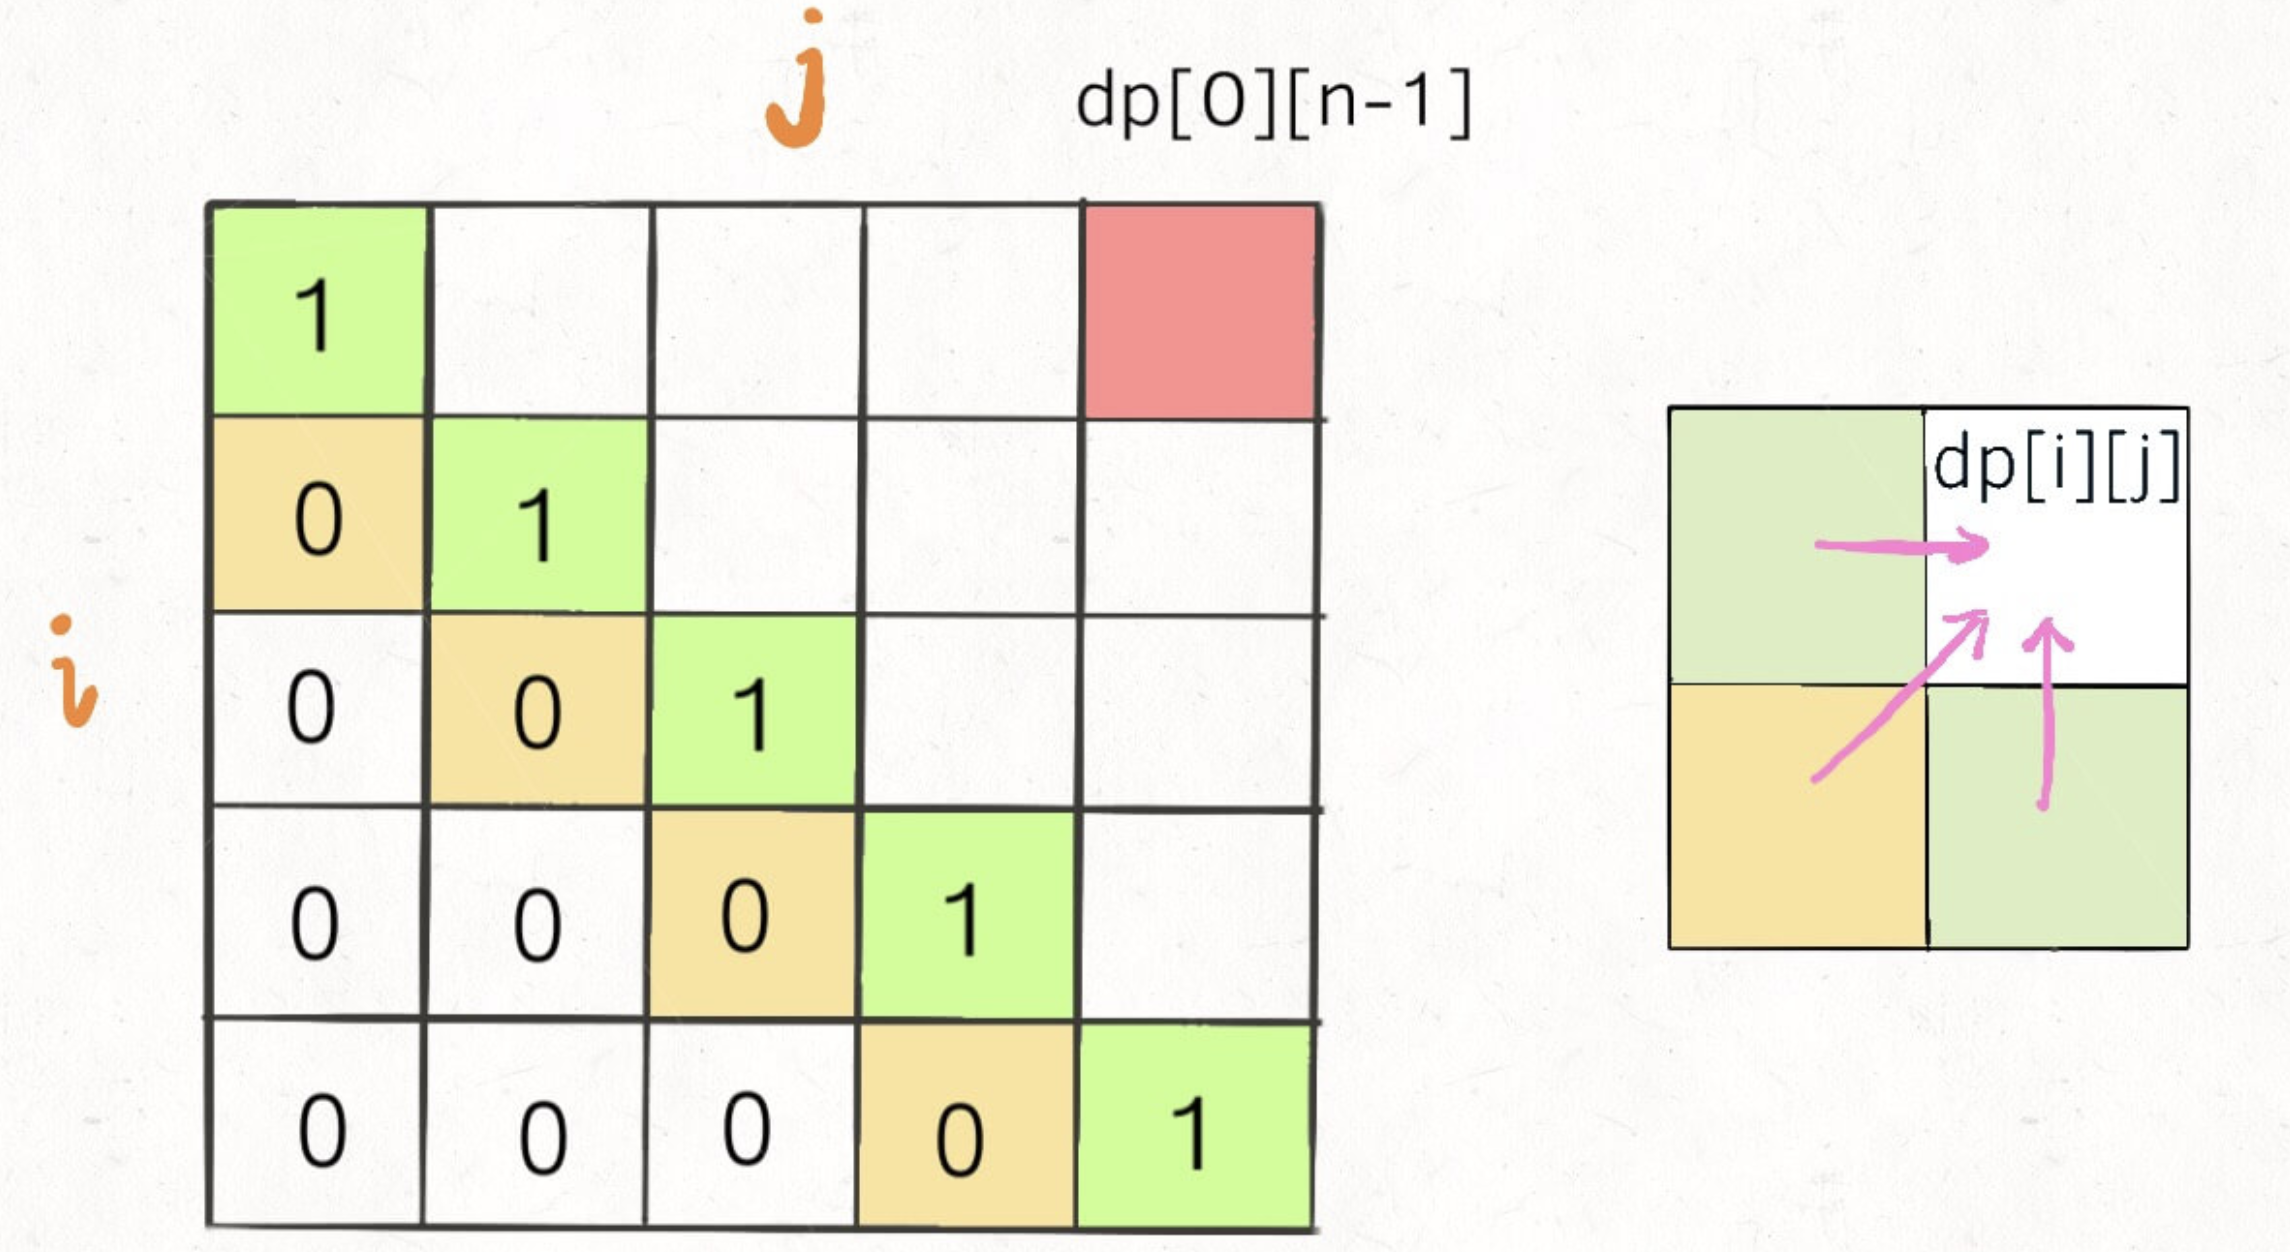
\includegraphics[width=1\textwidth]{fig/Dynamic_Programming_Longest_Recursive_Text_1.png}
\end{figure}

这种情况根据刚才的两个原则,就可以有两种正确的遍历方式:
\begin{figure}[H]
    \centering
    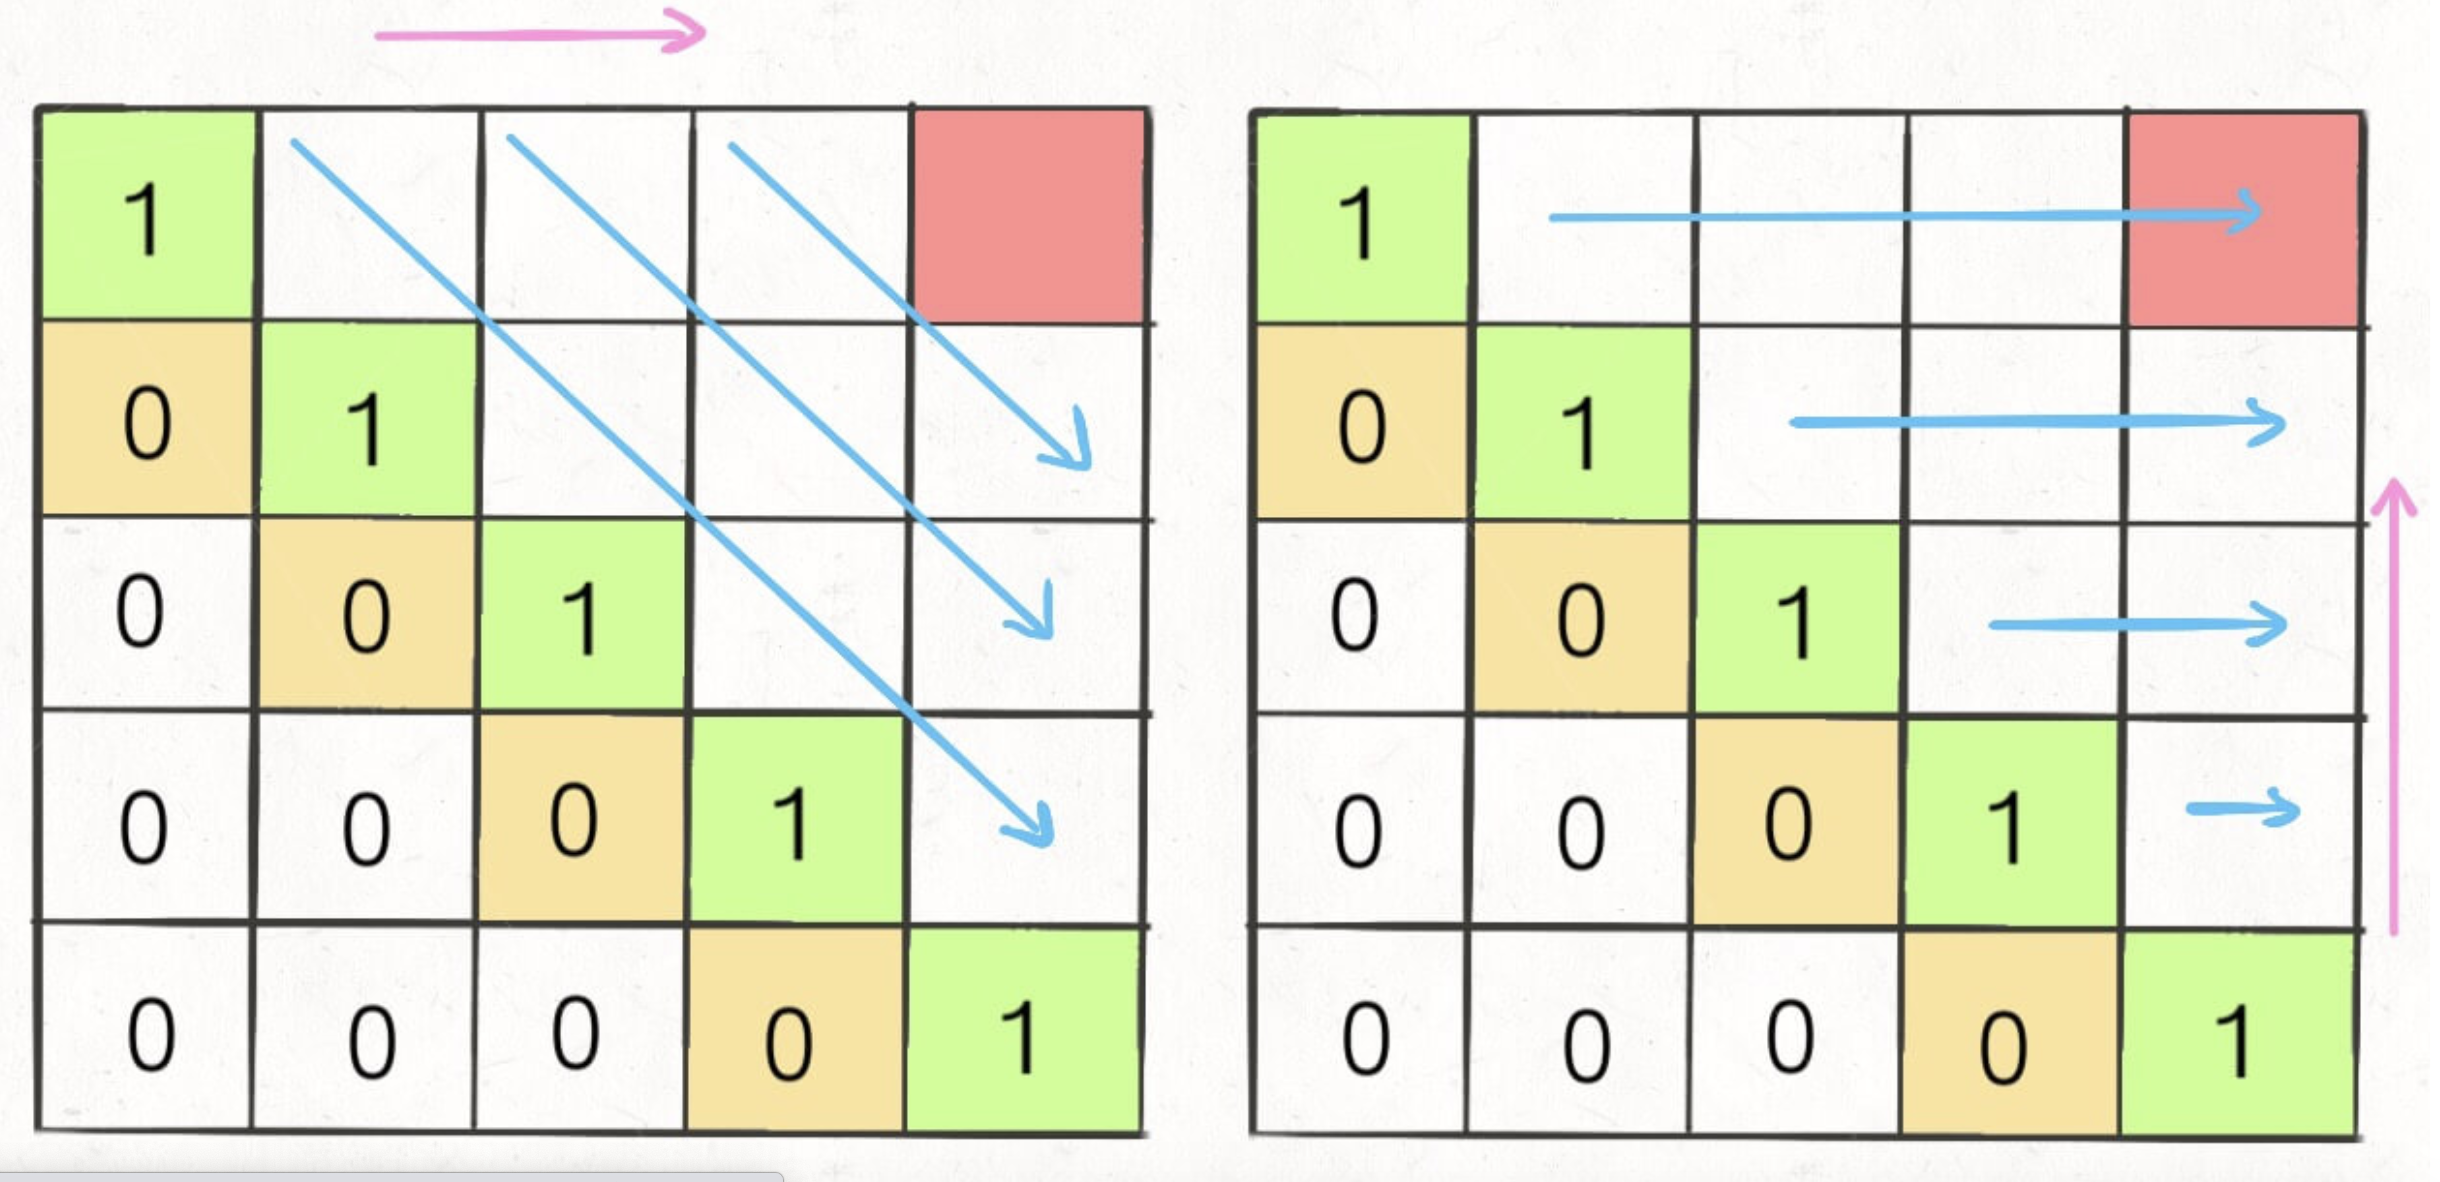
\includegraphics[width=1\textwidth]{fig/Dynamic_Programming_Longest_Recursive_Text_2.png}
\end{figure}

要么从左至右斜着遍历,要么从下向上从左到右遍历,这样才能保证每次 dp[i][j] 的左边、下边、左下边已经计算完毕,得到正确结果。

现在,你应该理解了这两个原则,主要就是看 base case 和最终结果的存储位置,保证遍历过程中使用的数据都是计算完毕的就行,有时候确实存在多种方法可以得到正确答案,可根据个人口味自行选择。

\section{相关题目}
\subsection{最长递增子序列}
\url{https://github.com/labuladong/fucking-algorithm/blob/master/%E5%8A%A8%E6%80%81%E8%A7%84%E5%88%92%E7%B3%BB%E5%88%97/%E5%8A%A8%E6%80%81%E8%A7%84%E5%88%92%E8%AE%BE%E8%AE%A1%EF%BC%9A%E6%9C%80%E9%95%BF%E9%80%92%E5%A2%9E%E5%AD%90%E5%BA%8F%E5%88%97.md}

最长递增子序列(Longest Increasing Subsequence,简写 LIS)是比较经典的一个问题,比较容易想到的是动态规划解法,时间复杂度 $O(N^2)$,我们借这个问题来由浅入深讲解如何写动态规划。比较难想到的是利用二分查找,时间复杂度是 $O(NlogN)$,我们通过一种简单的纸牌游戏来辅助理解这种巧妙的解法。

先看一下题目,很容易理解:
\begin{figure}[H]
    \centering
    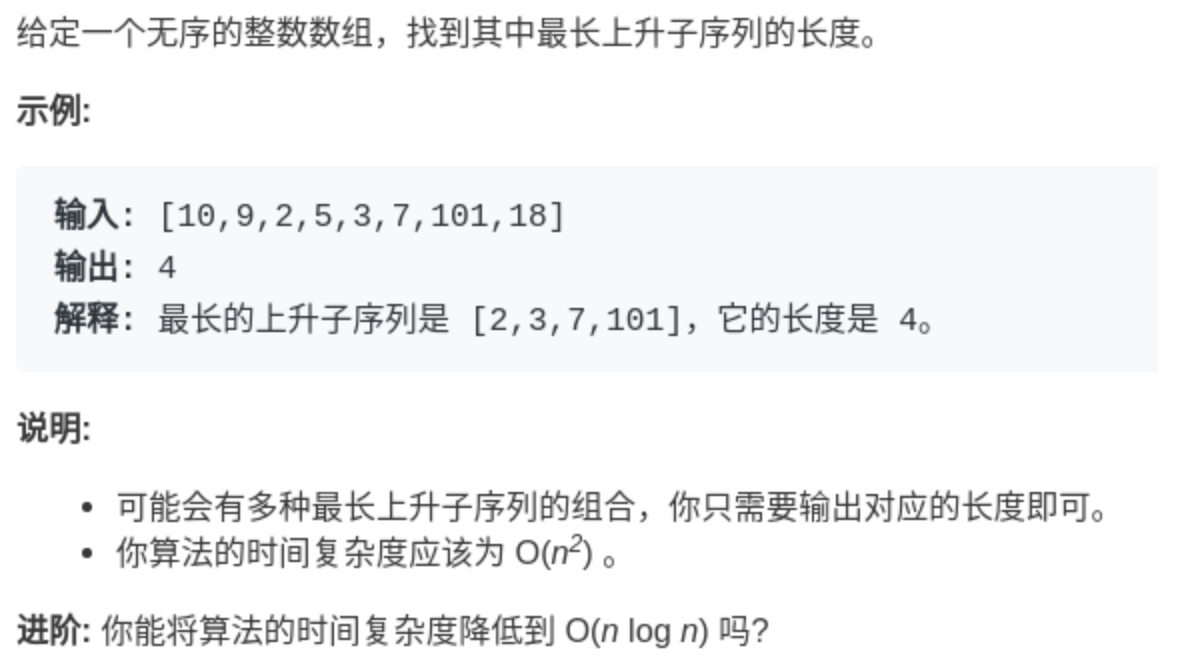
\includegraphics[width=.8\textwidth]{fig/Dynamic_Programming_Longest_Increasing Subsequence_1.png}
\end{figure}

\textbf{注意「子序列」和「子串」这两个名词的区别,子串一定是连续的,而子序列不一定是连续的}。下面先来一步一步设计动态规划算法解决这个问题。

\subsubsection{动态规划解法}
动态规划的核心设计思想是数学归纳法。

相信大家对数学归纳法都不陌生,高中就学过,而且思路很简单。比如我们想证明一个数学结论,那么我们先假设这个结论在 $k<n$ 时成立,然后想办法证明 $k=n$ 的时候此结论也成立。如果能够证明出来,那么就说明这个结论对于 k 等于任何数都成立。

类似的,我们设计动态规划算法,不是需要一个 dp 数组吗?我们可以假设 $dp[0...i-1]$ 都已经被算出来了,然后问自己:怎么通过这些结果算出 dp[i]?

直接拿最长递增子序列这个问题举例你就明白了。不过,首先要定义清楚 dp 数组的含义,即 dp[i] 的值到底代表着什么?

我们的定义是这样的:dp[i] 表示以 nums[i] 这个数结尾的最长递增子序列的长度。举两个例子:
\begin{figure}[H]
    \centering
    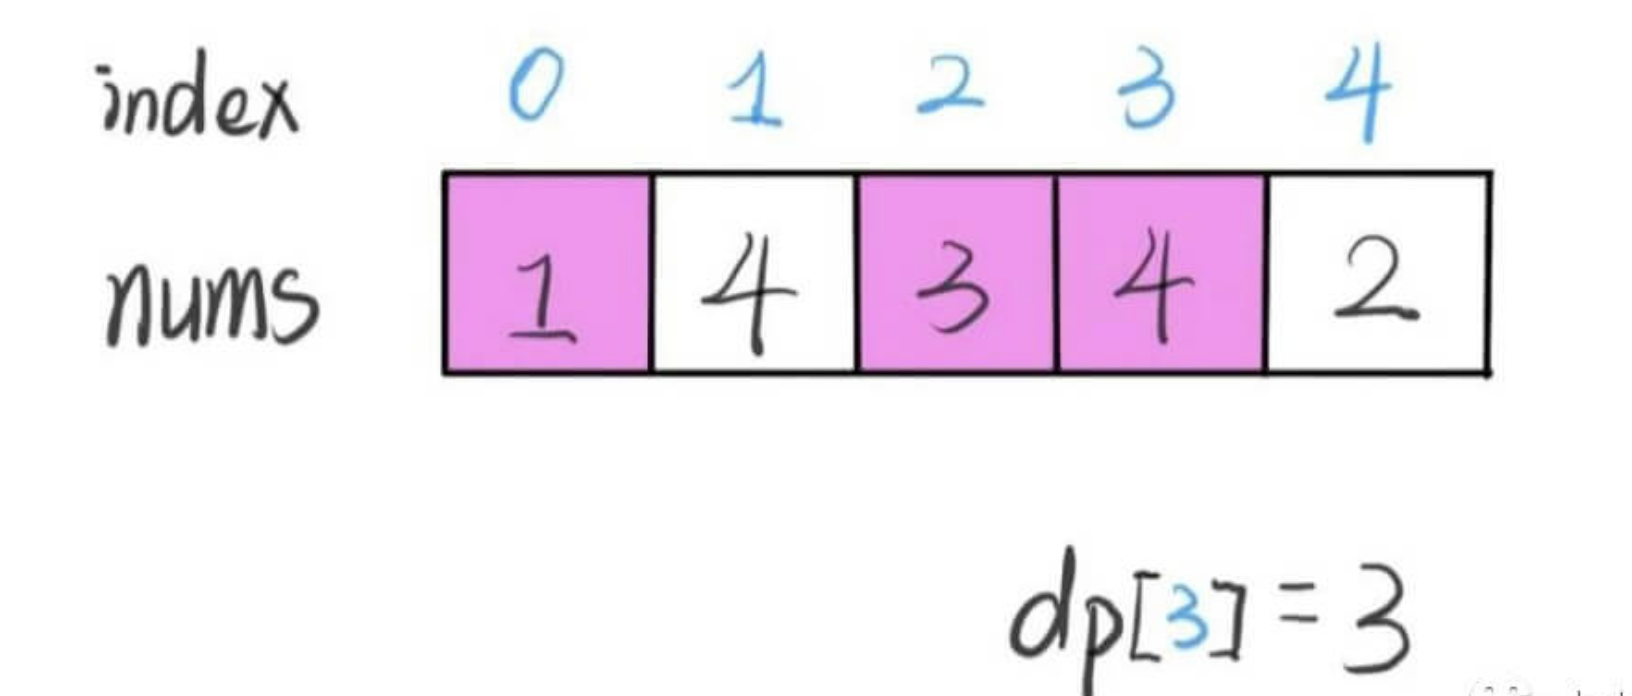
\includegraphics[width=.8\textwidth]{fig/Dynamic_Programming_Longest_Increasing Subsequence_2.png}
\end{figure}
\begin{figure}[H]
    \centering
    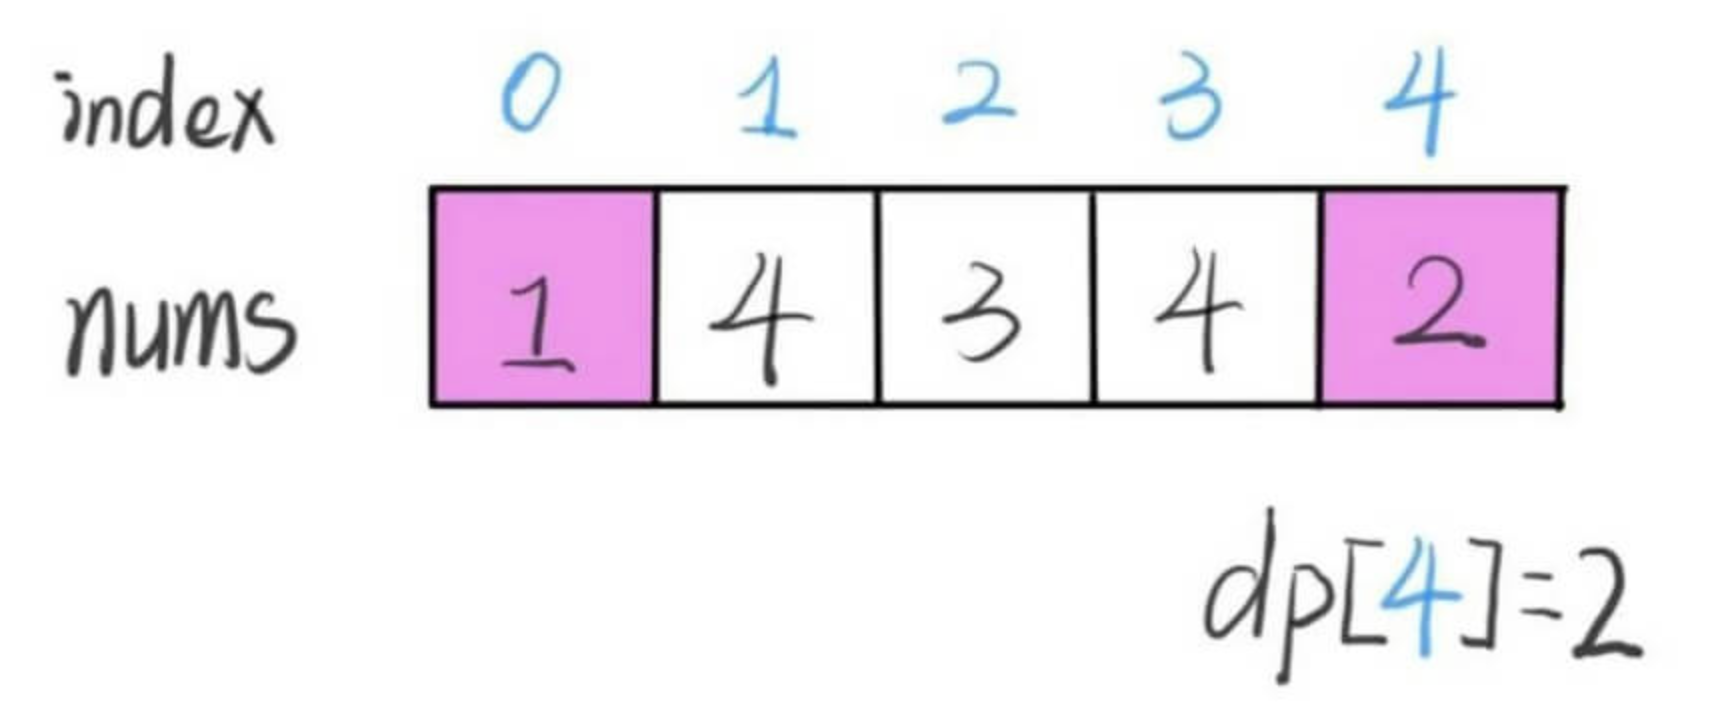
\includegraphics[width=.8\textwidth]{fig/Dynamic_Programming_Longest_Increasing Subsequence_3.png}
\end{figure}

算法演进的过程是这样的,:
\begin{figure}[H]
    \centering
    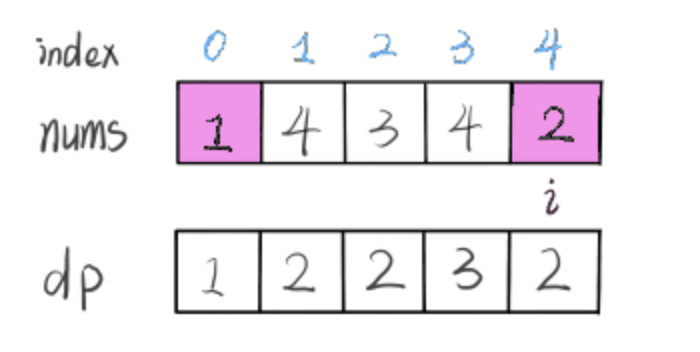
\includegraphics[width=.4\textwidth]{fig/Dynamic_Programming_Longest_Increasing Subsequence_4.png}
\end{figure}

根据这个定义,我们的最终结果(子序列的最大长度)应该是 dp 数组中的最大值。
\begin{lstlisting}
int res = 0;
for (int i = 0; i < dp.size(); i++) {
    res = Math.max(res, dp[i]);
}
return res;
\end{lstlisting}

读者也许会问,刚才这个过程中每个 dp[i] 的结果是我们肉眼看出来的,我们应该怎么设计算法逻辑来正确计算每个 dp[i] 呢?这就是动态规划的重头戏了,要思考如何进行状态转移,这里就可以使用数学归纳的思想:

我们已经知道了 $dp[0...4]$ 的所有结果,我们如何通过这些已知结果推出 $dp[5]$ 呢?
\begin{figure}[H]
    \centering
    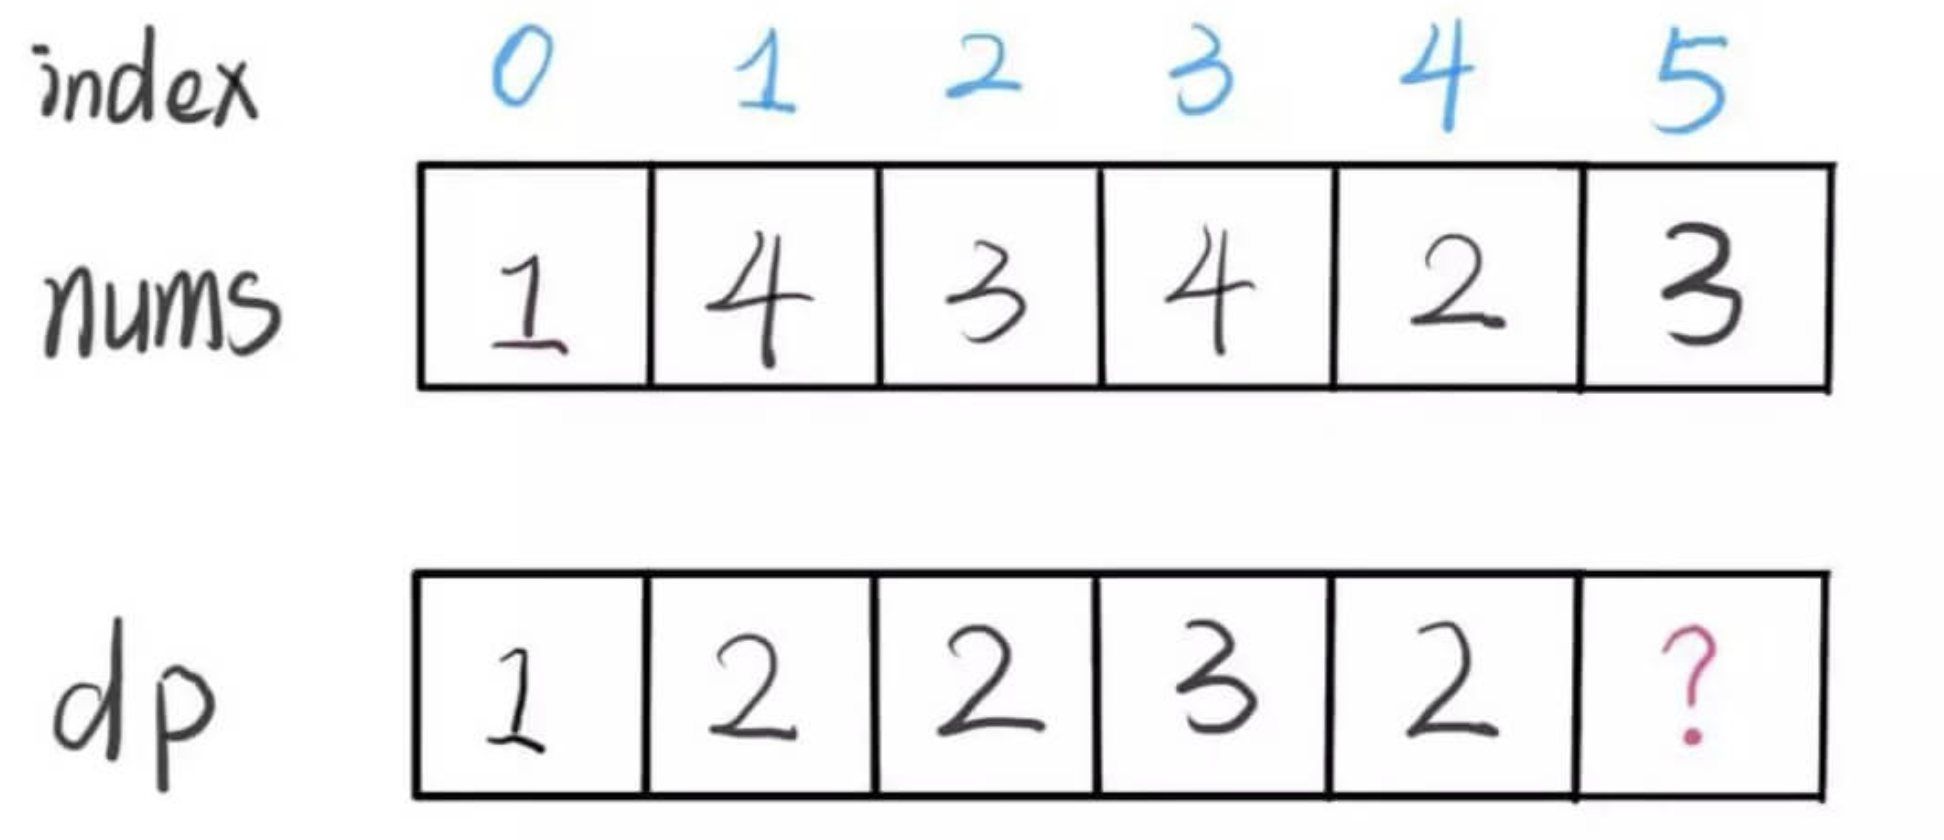
\includegraphics[width=.4\textwidth]{fig/Dynamic_Programming_Longest_Increasing Subsequence_5.png}
\end{figure}

根据刚才我们对 dp 数组的定义,现在想求 dp[5] 的值,也就是想求以 nums[5] 为结尾的最长递增子序列。

nums[5] = 3,既然是递增子序列,我们只要找到前面那些结尾比 3 小的子序列,然后把 3 接到最后,就可以形成一个新的递增子序列,而且这个新的子序列长度加一。

当然,可能形成很多种新的子序列,但是我们只要最长的,把最长子序列的长度作为 dp[5] 的值即可。
\begin{lstlisting}
for (int j = 0; j < i; j++) {
    if (nums[i] > nums[j]) 
        dp[i] = Math.max(dp[i], dp[j] + 1);
}
\end{lstlisting}

这段代码的逻辑就可以算出 dp[5]。到这里,这道算法题我们就基本做完了。读者也许会问,我们刚才只是算了 dp[5] 呀,dp[4], dp[3] 这些怎么算呢?类似数学归纳法,你已经可以算出 dp[5] 了,其他的就都可以算出来:
\begin{lstlisting}
for (int i = 0; i < nums.length; i++) {
    for (int j = 0; j < i; j++) {
        if (nums[i] > nums[j]) 
            dp[i] = Math.max(dp[i], dp[j] + 1);
    }
}
\end{lstlisting}

还有一个细节问题,dp 数组应该全部初始化为 1,因为子序列最少也要包含自己,所以长度最小为 1。下面我们看一下完整代码:
\begin{lstlisting}
public int lengthOfLIS(int[] nums) {
    int[] dp = new int[nums.length];
    // dp 数组全都初始化为 1
    Arrays.fill(dp, 1);
    for (int i = 0; i < nums.length; i++) {
        for (int j = 0; j < i; j++) {
            if (nums[i] > nums[j]) 
                dp[i] = Math.max(dp[i], dp[j] + 1);
        }
    }
    
    int res = 0;
    for (int i = 0; i < dp.length; i++) {
        res = Math.max(res, dp[i]);
    }
    return res;
}
\end{lstlisting}
至此,这道题就解决了,时间复杂度 $O(N^2)$。总结一下动态规划的设计流程:

首先明确 dp 数组所存数据的含义。这步很重要,如果不得当或者不够清晰,会阻碍之后的步骤。

然后根据 dp 数组的定义,运用数学归纳法的思想,假设 $dp[0...i-1]$ 都已知,想办法求出 $dp[i]$,一旦这一步完成,整个题目基本就解决了。

但如果无法完成这一步,很可能就是 dp 数组的定义不够恰当,需要重新定义 dp 数组的含义;或者可能是 dp 数组存储的信息还不够,不足以推出下一步的答案,需要把 dp 数组扩大成二维数组甚至三维数组。

最后想一想问题的 base case 是什么,以此来初始化 dp 数组,以保证算法正确运行。

\subsubsection{二分查找解法}
这个解法的时间复杂度会将为 O(NlogN),但是说实话,正常人基本想不到这种解法(也许玩过某些纸牌游戏的人可以想出来)。所以如果大家了解一下就好,正常情况下能够给出动态规划解法就已经很不错了。

根据题目的意思,我都很难想象这个问题竟然能和二分查找扯上关系。其实最长递增子序列和一种叫做 patience game 的纸牌游戏有关,甚至有一种排序方法就叫做 patience sorting(耐心排序)。

为了简单起见,后文跳过所有数学证明,通过一个简化的例子来理解一下思路。

首先,给你一排扑克牌,我们像遍历数组那样从左到右一张一张处理这些扑克牌,最终要把这些牌分成若干堆。
\begin{figure}[H]
    \centering
    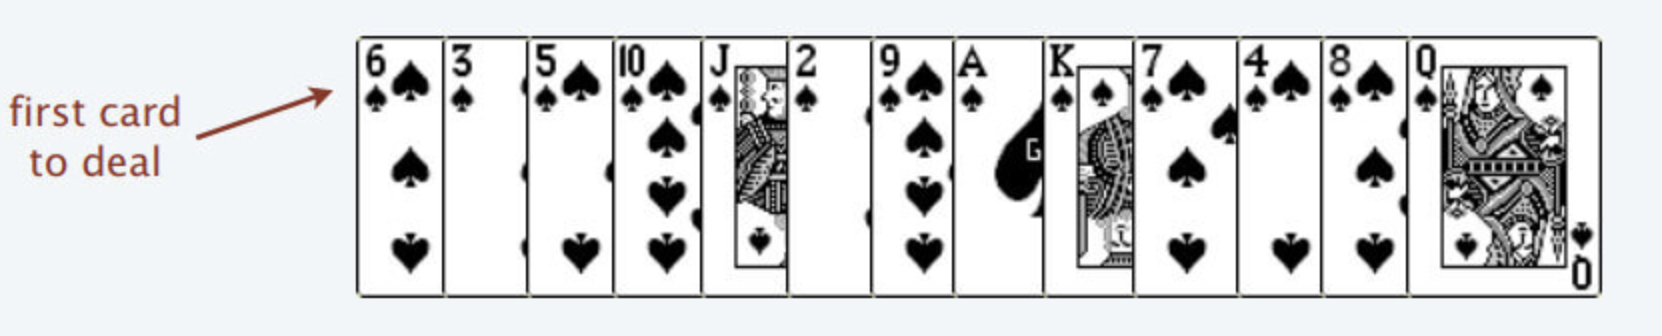
\includegraphics[width=1\textwidth]{fig/Dynamic_Programming_Longest_Increasing Subsequence_6.png}
\end{figure}

处理这些扑克牌要遵循以下规则:只能把点数小的牌压到点数比它大的牌上。如果当前牌点数较大没有可以放置的堆,则新建一个堆,把这张牌放进去。如果当前牌有多个堆可供选择,则选择最左边的堆放置。

比如说上述的扑克牌最终会被分成这样 5 堆(我们认为 A 的值是最大的,而不是 1)。
\begin{figure}[H]
    \centering
    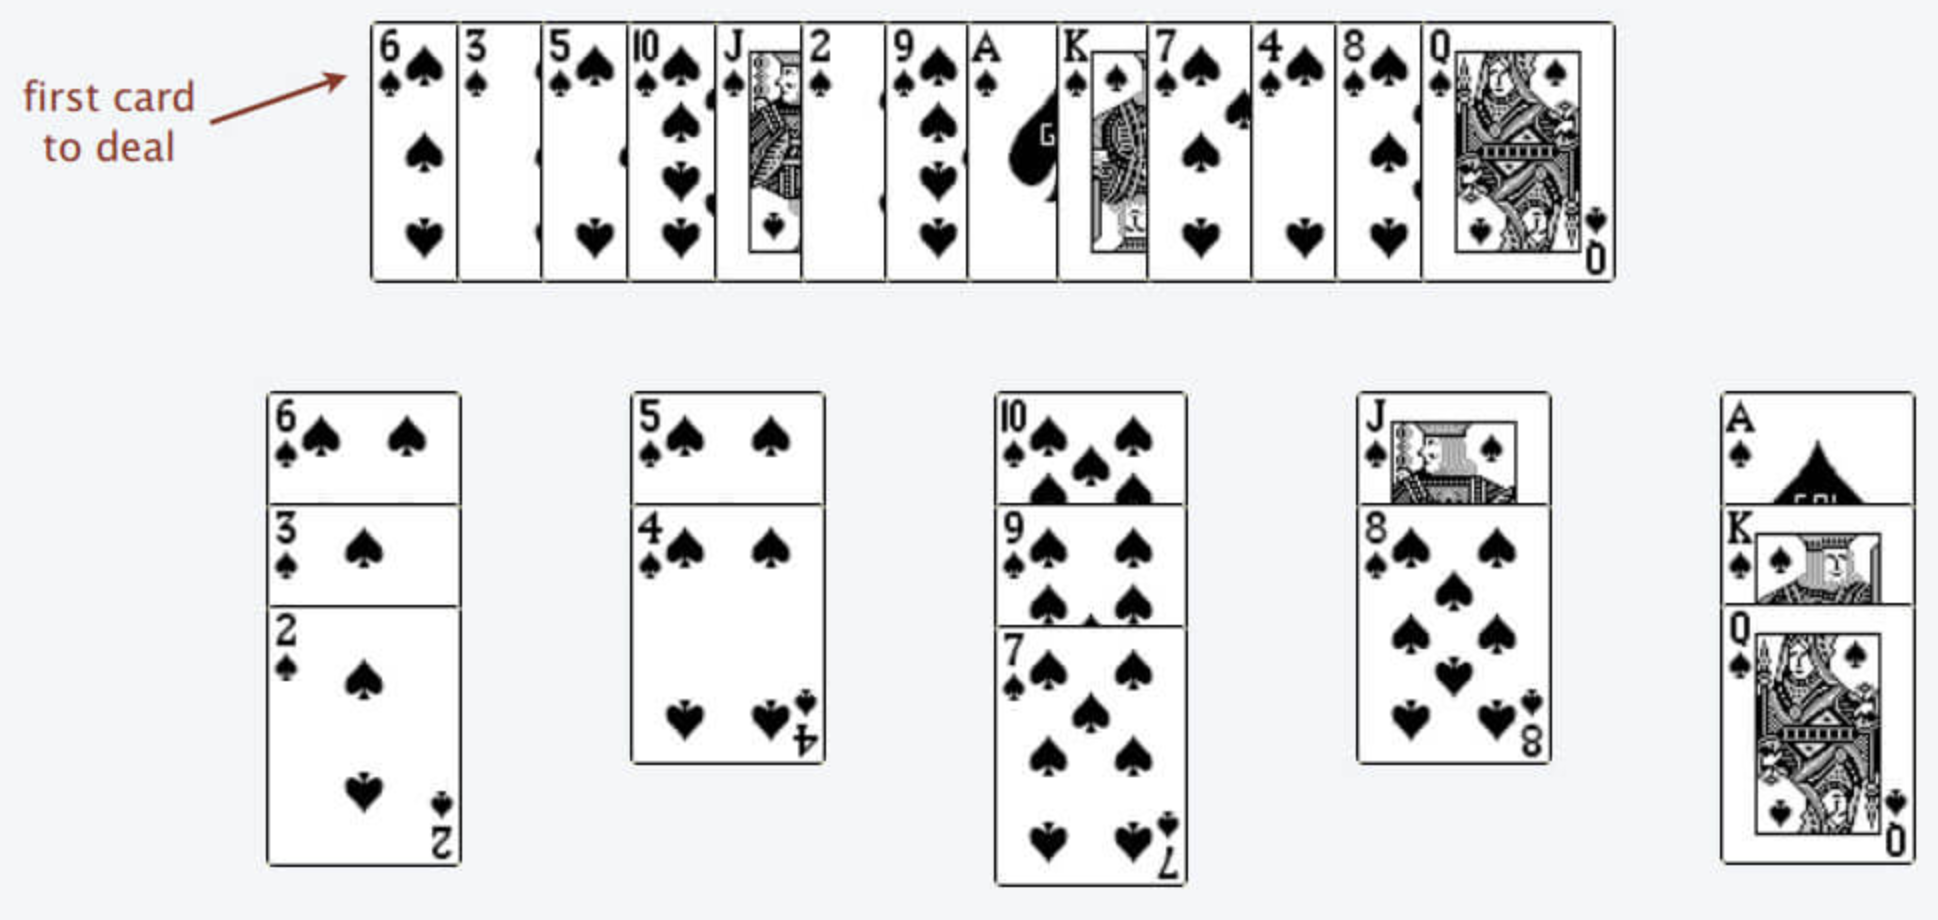
\includegraphics[width=1\textwidth]{fig/Dynamic_Programming_Longest_Increasing Subsequence_7.png}
\end{figure}

为什么遇到多个可选择堆的时候要放到最左边的堆上呢?因为这样可以保证牌堆顶的牌有序(2, 4, 7, 8, Q),证明略。
\begin{figure}[H]
    \centering
    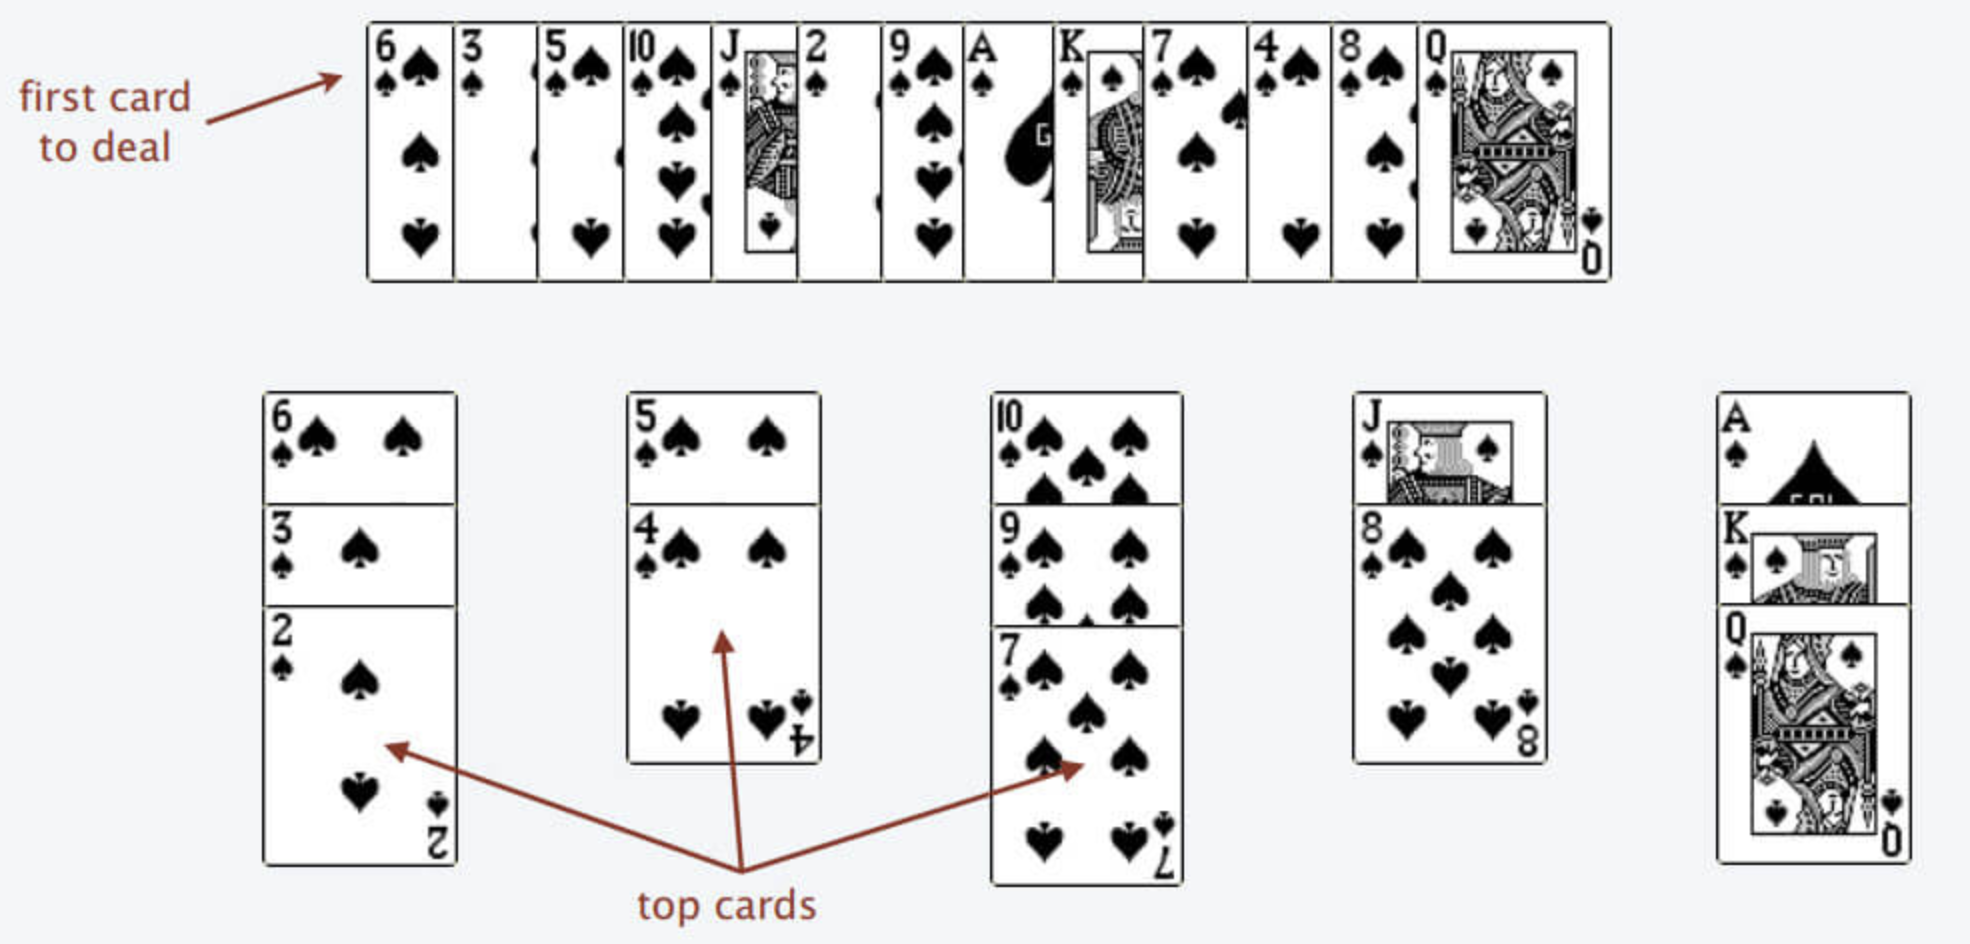
\includegraphics[width=1\textwidth]{fig/Dynamic_Programming_Longest_Increasing Subsequence_8.png}
\end{figure}

按照上述规则执行,可以算出最长递增子序列,牌的堆数就是最长递增子序列的长度,证明略。
\begin{figure}[H]
    \centering
    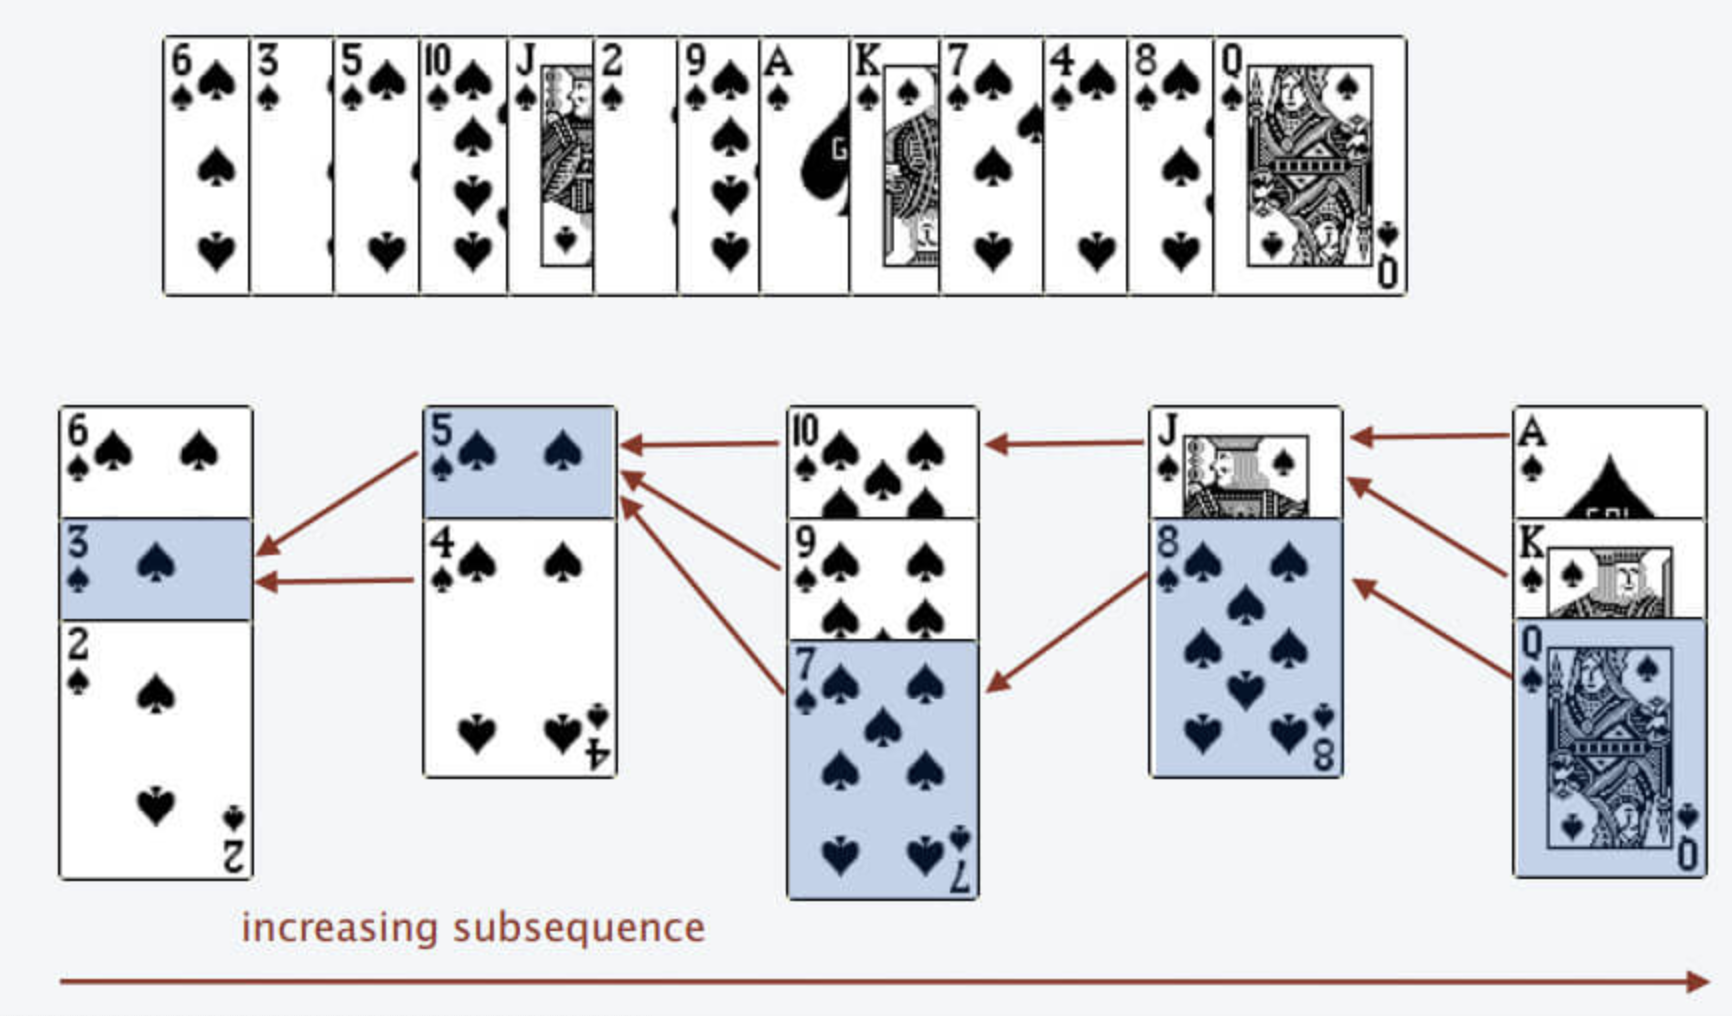
\includegraphics[width=1\textwidth]{fig/Dynamic_Programming_Longest_Increasing Subsequence_9.png}
\end{figure}
我们只要把处理扑克牌的过程编程写出来即可。每次处理一张扑克牌不是要找一个合适的牌堆顶来放吗,牌堆顶的牌不是有序吗,这就能用到二分查找了:用二分查找来搜索当前牌应放置的位置。
\begin{lstlisting}
public int lengthOfLIS(int[] nums) {
    int[] top = new int[nums.length];
    // 牌堆数初始化为 0
    int piles = 0;
    for (int i = 0; i < nums.length; i++) {
        // 要处理的扑克牌
        int poker = nums[i];

        /***** 搜索左侧边界的二分查找 *****/
        int left = 0, right = piles;
        while (left < right) {
            int mid = (left + right) / 2;
            if (top[mid] > poker) {
                right = mid;
            } else if (top[mid] < poker) {
                left = mid + 1;
            } else {
                right = mid;
            }
        }
        /*********************************/
        
        // 没找到合适的牌堆,新建一堆
        if (left == piles) piles++;
        // 把这张牌放到牌堆顶
        top[left] = poker;
    }
    // 牌堆数就是 LIS 长度
    return piles;
}
\end{lstlisting}

\subsection{编辑距离}
\begin{figure}[H]
    \centering
    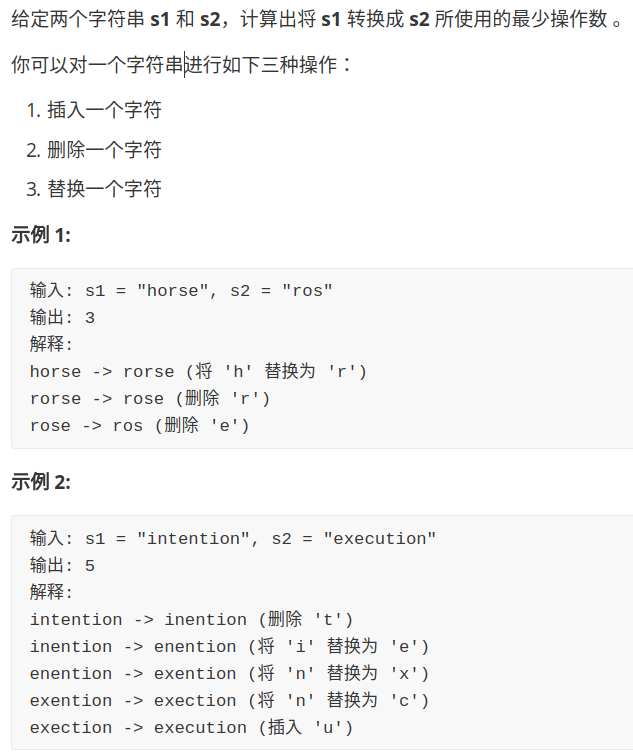
\includegraphics[width=.8\textwidth]{fig/Dynamic_Programming_Edit_Distance_1.png}
\end{figure}
举个该问题的应用:DNA 序列是由 A,G,C,T 组成的序列,可以类比成字符串。编辑距离可以衡量两个 DNA 序列的相似度,编辑距离越小,说明这两段 DNA 越相似,说不定这俩 DNA 的主人是远古近亲啥的。
\subsubsection{思路}
编辑距离问题就是给我们两个字符串 s1 和 s2,只能用三种操作,让我们把 s1 变成 s2,求最少的操作数。需要明确的是,不管是把 s1 变成 s2 还是反过来,结果都是一样的,所以后文就以 s1 变成 s2 举例。

前文「最长公共子序列」说过,解决两个字符串的动态规划问题,一般都是用两个指针 i,j 分别指向两个字符串的最后,然后一步步往前走,缩小问题的规模。

base case 是 i 走完 s1 或 j 走完 s2,可以直接返回另一个字符串剩下的长度。

对于每对儿字符 s1[i] 和 s2[j],可以有四种操作:
\begin{lstlisting}
if s1[i] == s2[j]:
    啥都别做(skip)
    i, j 同时向前移动
else:
    三选一:
        插入(insert)
        删除(delete)
        替换(replace)
\end{lstlisting}

有这个框架,问题就已经解决了。读者也许会问,这个「三选一」到底该怎么选择呢?很简单,全试一遍,哪个操作最后得到的编辑距离最小,就选谁。这里需要递归技巧,理解需要点技巧,先看下代码:
\begin{lstlisting}
def minDistance(s1, s2) -> int:

    def dp(i, j):
        # base case
        if i == -1: return j + 1
        if j == -1: return i + 1
        
        if s1[i] == s2[j]:
            return dp(i - 1, j - 1)  # 啥都不做
        else:
            return min(
                dp(i, j - 1) + 1,    # 插入
                dp(i - 1, j) + 1,    # 删除
                dp(i - 1, j - 1) + 1 # 替换
            )
    
    # i,j 初始化指向最后一个索引
    return dp(len(s1) - 1, len(s2) - 1)
\end{lstlisting}

下面来详细解释一下这段递归代码,base case 应该不用解释了,主要解释一下递归部分。

都说递归代码的可解释性很好,这是有道理的,只要理解函数的定义,就能很清楚地理解算法的逻辑。我们这里 dp(i, j) 函数的定义是这样的:
\begin{lstlisting}
def dp(i, j) -> int
# 返回 s1[0..i] 和 s2[0..j] 的最小编辑距离
\end{lstlisting}

记住这个定义之后,先来看这段代码:
\begin{lstlisting}
if s1[i] == s2[j]:
    return dp(i - 1, j - 1)  # 啥都不做
# 解释:
# 本来就相等,不需要任何操作
# s1[0..i] 和 s2[0..j] 的最小编辑距离等于
# s1[0..i-1] 和 s2[0..j-1] 的最小编辑距离
# 也就是说 dp(i, j) 等于 dp(i-1, j-1)
\end{lstlisting}

如果 s1[i]!=s2[j],就要对三个操作递归了,稍微需要点思考:
\begin{lstlisting}
dp(i, j - 1) + 1,    # 插入
# 解释:
# 我直接在 s1[i] 插入一个和 s2[j] 一样的字符
# 那么 s2[j] 就被匹配了,前移 j,继续跟 i 对比
# 别忘了操作数加一
\end{lstlisting}

\begin{lstlisting}
dp(i - 1, j) + 1,    # 删除
# 解释:
# 我直接把 s[i] 这个字符删掉
# 前移 i,继续跟 j 对比
# 操作数加一
\end{lstlisting}

\begin{lstlisting}
dp(i - 1, j - 1) + 1 # 替换
# 解释:
# 我直接把 s1[i] 替换成 s2[j],这样它俩就匹配了
# 同时前移 i,j 继续对比
# 操作数加一
\end{lstlisting}

现在,你应该完全理解这段短小精悍的代码了。还有点小问题就是,这个解法是暴力解法,存在重叠子问题,需要用动态规划技巧来优化。

怎么能一眼看出存在重叠子问题呢?需要抽象出本文算法的递归框架:
\begin{lstlisting}
def dp(i, j):
    dp(i - 1, j - 1) #1
    dp(i, j - 1)     #2
    dp(i - 1, j)     #3
\end{lstlisting}

对于子问题 dp(i-1, j-1),如何通过原问题 dp(i, j) 得到呢?有不止一条路径,比如 dp(i, j) -> \#1 和 dp(i, j) -> \#2 -> \#3。一旦发现一条重复路径,就说明存在巨量重复路径,也就是重叠子问题。

\subsubsection{动态规划优化}
对于重叠子问题呢,前文「动态规划详解」详细介绍过,优化方法无非是备忘录或者 DP table。

备忘录很好加,原来的代码稍加修改即可:
\begin{lstlisting}
def minDistance(s1, s2) -> int:

    memo = dict() # 备忘录
    def dp(i, j):
        if (i, j) in memo: 
            return memo[(i, j)]
        ...
        
        if s1[i] == s2[j]:
            memo[(i, j)] = ...  
        else:
            memo[(i, j)] = ...
        return memo[(i, j)]
    
    return dp(len(s1) - 1, len(s2) - 1)
\end{lstlisting}

主要说下 DP table 的解法:首先明确 dp 数组的含义,dp 数组是一个二维数组,长这样:
\begin{figure}[H]
    \centering
    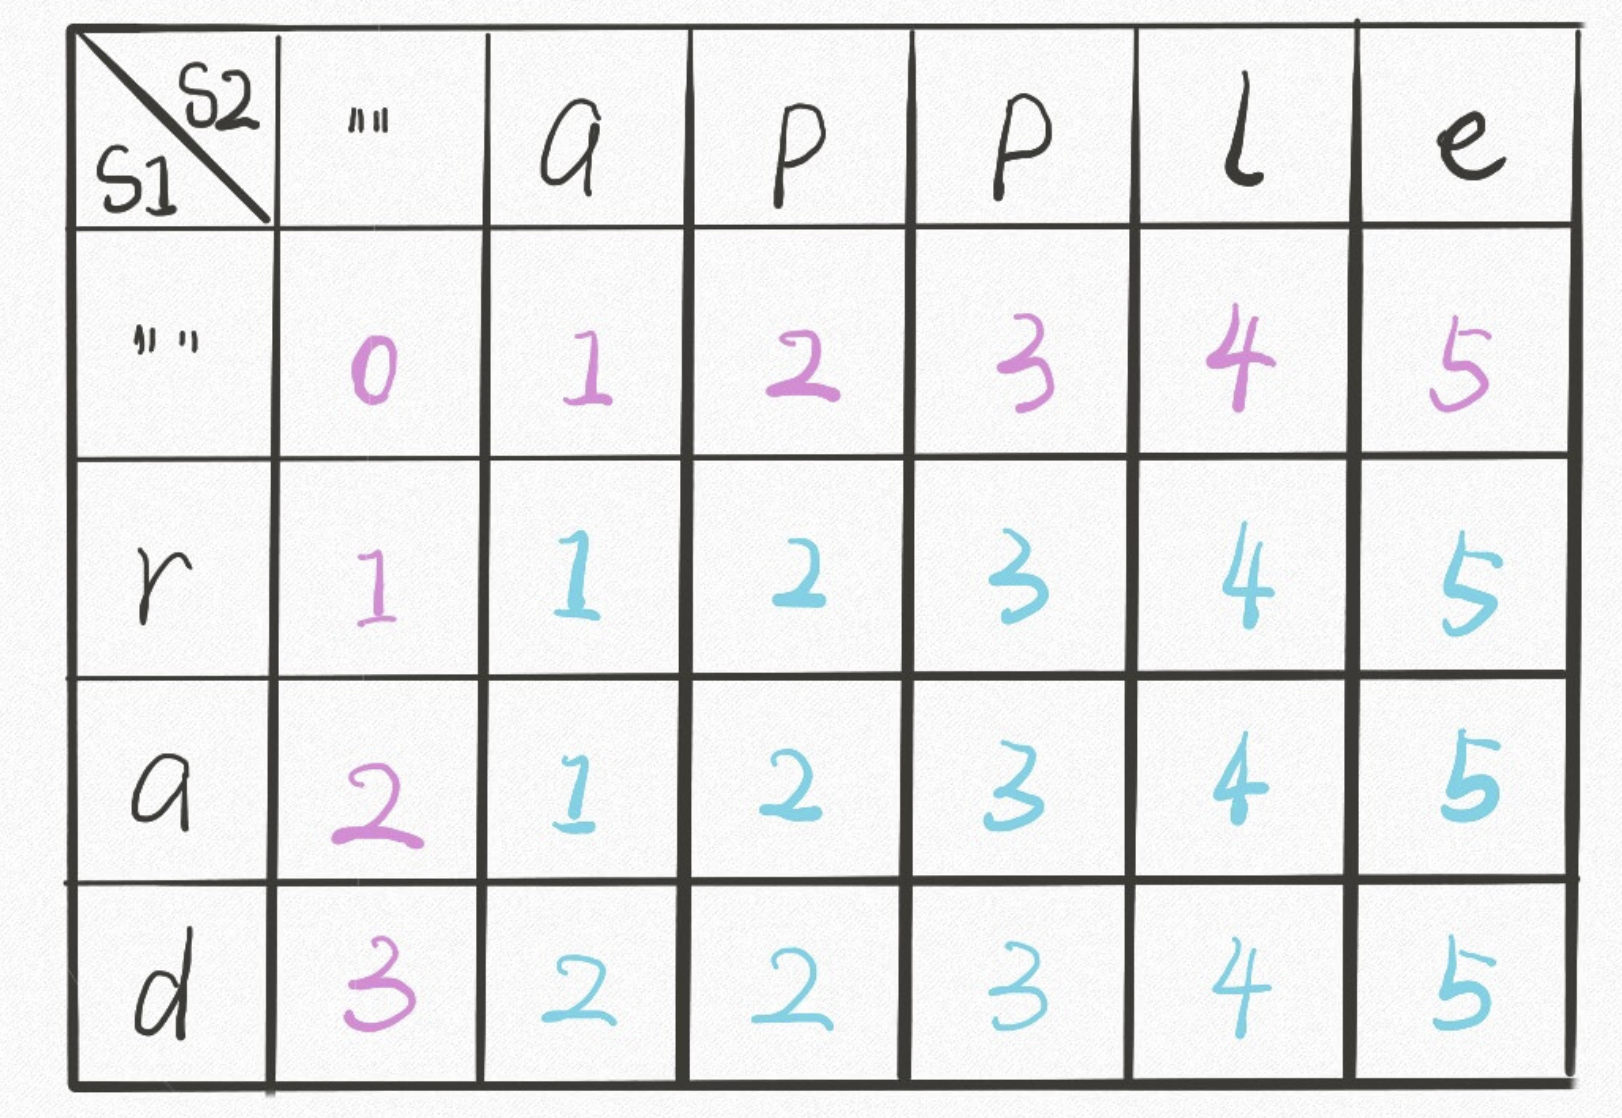
\includegraphics[width=.6\textwidth]{fig/Dynamic_Programming_Edit_Distance_2.png}
\end{figure}

有了之前递归解法的铺垫,应该很容易理解。dp[..][0] 和 dp[0][..] 对应 base case,dp[i][j] 的含义和之前的 dp 函数类似:
\begin{lstlisting}
def dp(i, j) -> int
# 返回 s1[0..i] 和 s2[0..j] 的最小编辑距离

dp[i-1][j-1]
# 存储 s1[0..i] 和 s2[0..j] 的最小编辑距离
\end{lstlisting}

dp 函数的 base case 是 i,j 等于 -1,而数组索引至少是 0,所以 dp 数组会偏移一位。

既然 dp 数组和递归 dp 函数含义一样,也就可以直接套用之前的思路写代码,唯一不同的是,DP table 是自底向上求解,递归解法是自顶向下求解:
\begin{lstlisting}
int minDistance(String s1, String s2) {
    int m = s1.length(), n = s2.length();
    int[][] dp = new int[m + 1][n + 1];
    // base case 
    for (int i = 1; i <= m; i++)
        dp[i][0] = i;
    for (int j = 1; j <= n; j++)
        dp[0][j] = j;
    // 自底向上求解
    for (int i = 1; i <= m; i++)
        for (int j = 1; j <= n; j++)
            if (s1.charAt(i-1) == s2.charAt(j-1))
                dp[i][j] = dp[i - 1][j - 1];
            else               
                dp[i][j] = min(
                    dp[i - 1][j] + 1,
                    dp[i][j - 1] + 1,
                    dp[i-1][j-1] + 1
                );
    // 储存着整个 s1 和 s2 的最小编辑距离
    return dp[m][n];
}

int min(int a, int b, int c) {
    return Math.min(a, Math.min(b, c));
}
\end{lstlisting}

\subsubsection{扩展延伸}
一般来说,处理两个字符串的动态规划问题,都是按本文的思路处理,建立 DP table。为什么呢,因为易于找出状态转移的关系,比如编辑距离的 DP table:

\begin{figure}[H]
    \centering
    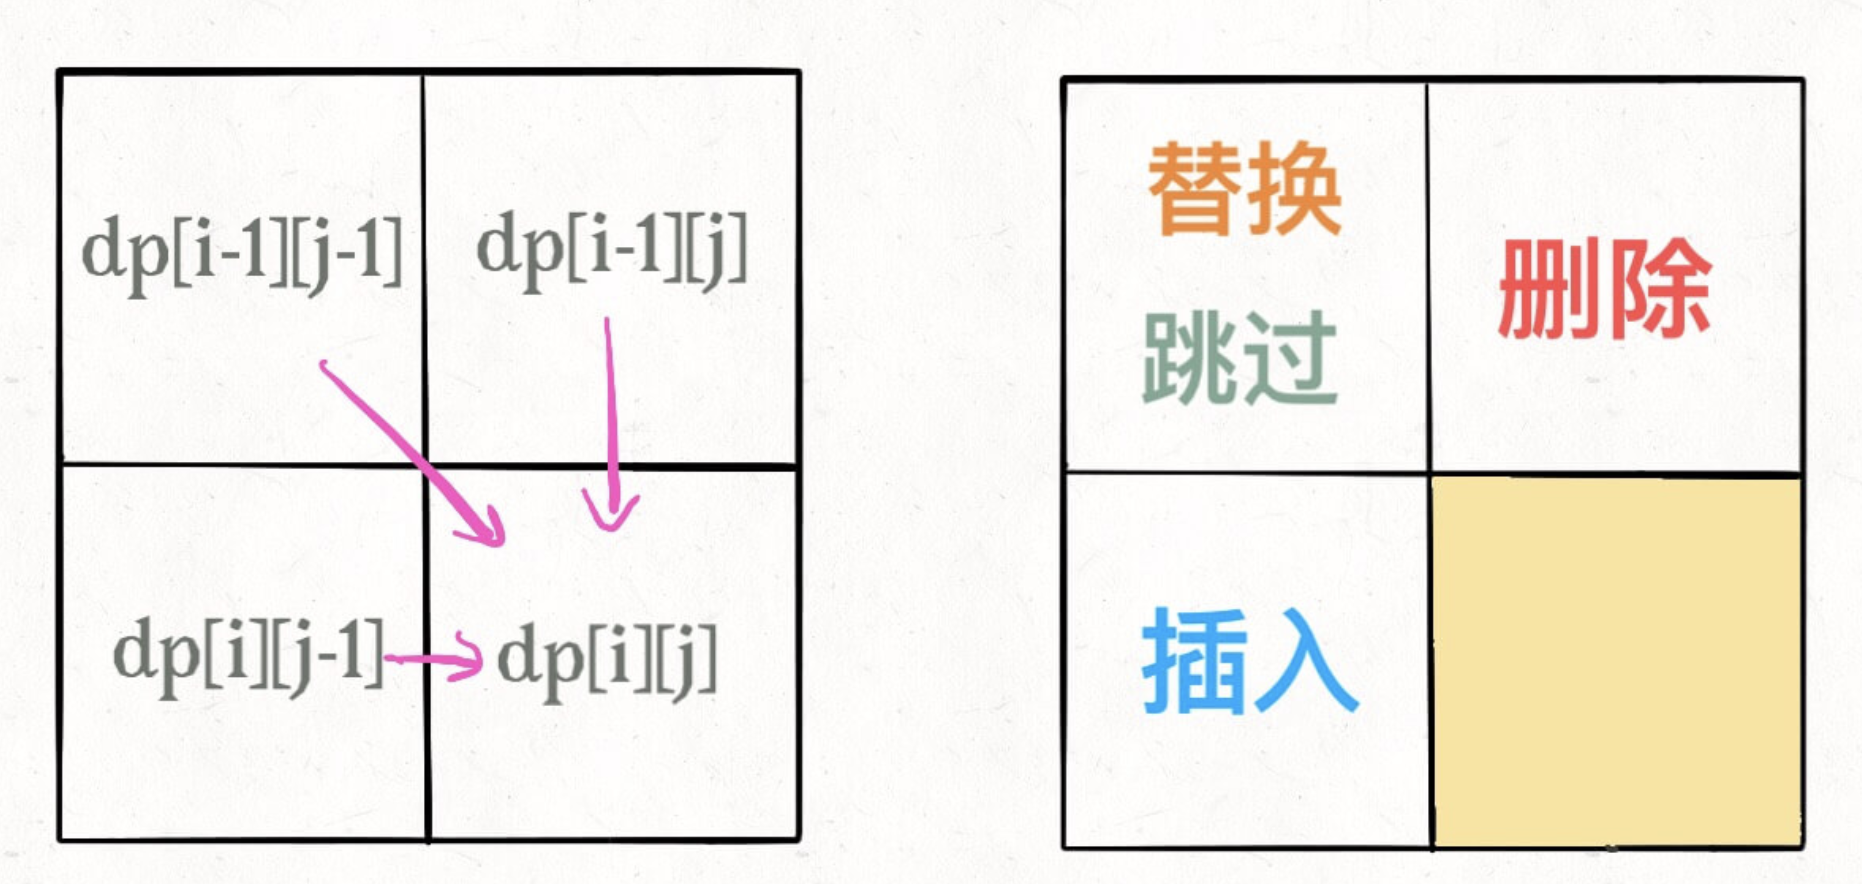
\includegraphics[width=.6\textwidth]{fig/Dynamic_Programming_Edit_Distance_3.png}
\end{figure}

还有一个细节,既然每个 dp[i][j] 只和它附近的三个状态有关,空间复杂度是可以压缩成 $O(min(M, N))$ 的(M,N 是两个字符串的长度)。不难,但是可解释性大大降低,读者可以自己尝试优化一下。

你可能还会问,这里只求出了最小的编辑距离,那具体的操作是什么?你之前举的修改公众号文章的例子,只有一个最小编辑距离肯定不够,还得知道具体怎么修改才行。

这个其实很简单,代码稍加修改,给 dp 数组增加额外的信息即可:
\begin{lstlisting}
// int[][] dp;
Node[][] dp;

class Node {
    int val;
    int choice;
    // 0 代表啥都不做
    // 1 代表插入
    // 2 代表删除
    // 3 代表替换
}
\end{lstlisting}

val 属性就是之前的 dp 数组的数值,choice 属性代表操作。在做最优选择时,顺便把操作记录下来,然后就从结果反推具体操作。

我们的最终结果不是 dp[m][n] 吗,这里的 val 存着最小编辑距离,choice 存着最后一个操作,比如说是插入操作,那么就可以左移一格:
\begin{figure}[H]
    \centering
    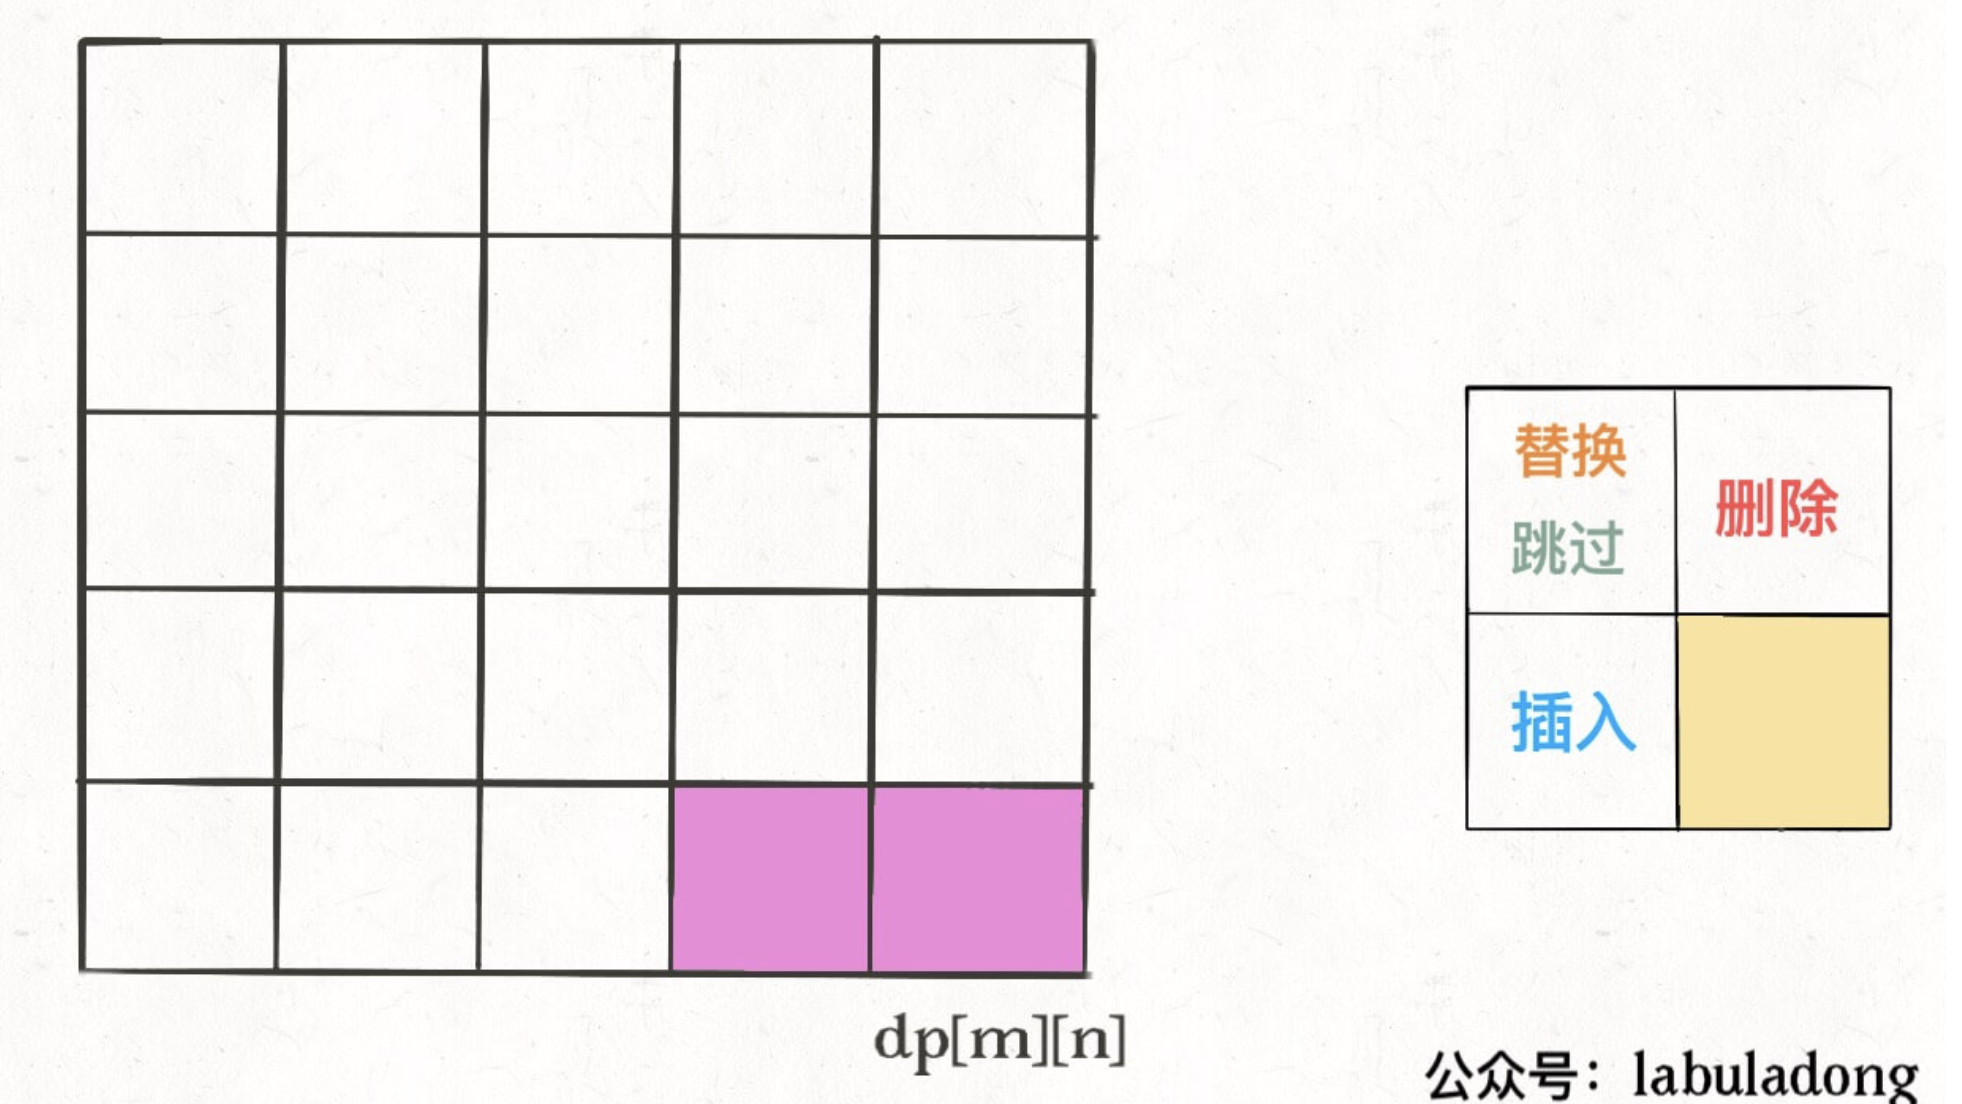
\includegraphics[width=.6\textwidth]{fig/Dynamic_Programming_Edit_Distance_4.png}
\end{figure}

重复此过程,可以一步步回到起点 dp[0][0],形成一条路径,按这条路径上的操作进行编辑,就是最佳方案。
\begin{figure}[H]
    \centering
    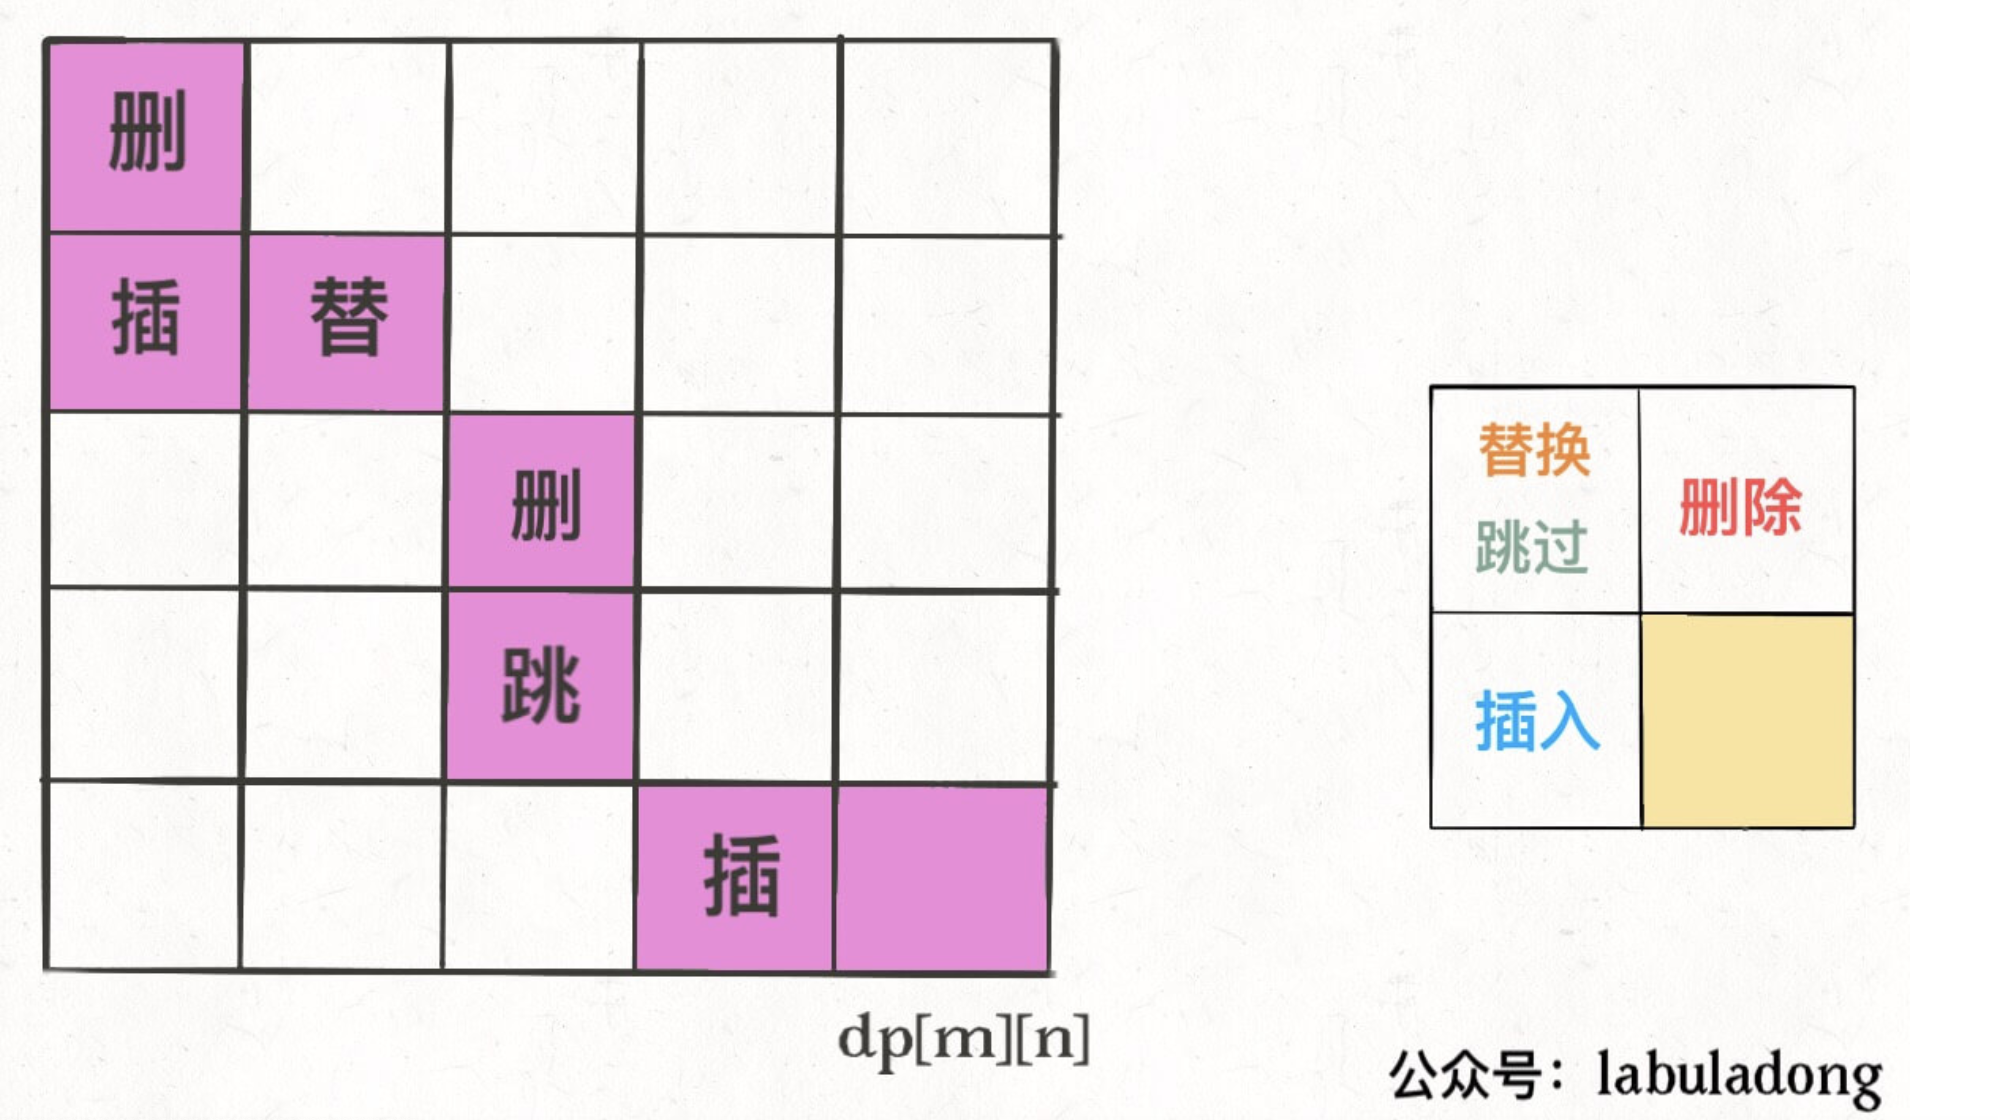
\includegraphics[width=.6\textwidth]{fig/Dynamic_Programming_Edit_Distance_5.png}
\end{figure}

\subsection{高楼扔鸡蛋}
\url{https://github.com/labuladong/fucking-algorithm/blob/master/%E5%8A%A8%E6%80%81%E8%A7%84%E5%88%92%E7%B3%BB%E5%88%97/%E9%AB%98%E6%A5%BC%E6%89%94%E9%B8%A1%E8%9B%8B%E9%97%AE%E9%A2%98.md}

\subsubsection{问题描述和解析}
题目:你面前有一栋从 1 到 N 共 N 层的楼,然后给你 K 个鸡蛋(K 至少为 1)。现在确定这栋楼存在楼层 0 <= F <= N,在这层楼将鸡蛋扔下去,鸡蛋恰好没摔碎(高于 F 的楼层都会碎,低于 F 的楼层都不会碎)。现在问你,最坏情况下,你至少要扔几次鸡蛋,才能确定这个楼层 F 呢?

也就是让你找摔不碎鸡蛋的最高楼层 F,但什么叫「最坏情况」下「至少」要扔几次呢?我们分别举个例子就明白了。

比方说现在先不管鸡蛋个数的限制,有 7 层楼,你怎么去找鸡蛋恰好摔碎的那层楼?最原始的方式就是线性扫描:我先在 1 楼扔一下,没碎,我再去 2 楼扔一下,没碎,我再去 3 楼……以这种策略,最坏情况应该就是我试到第 7 层鸡蛋也没碎(F = 7),也就是我扔了 7 次鸡蛋。

现在你应该理解什么叫做「最坏情况」下了,鸡蛋破碎一定发生在搜索区间穷尽时,不会说你在第 1 层摔一下鸡蛋就碎了,这是你运气好,不是最坏情况。

现在再来理解一下什么叫「至少」要扔几次。依然不考虑鸡蛋个数限制,同样是 7 层楼,我们可以优化策略。最好的策略是使用二分查找思路,我先去第 (1 + 7) / 2 = 4 层扔一下:如果碎了说明 F 小于 4,我就去第 (1 + 3) / 2 = 2 层试……;如果没碎说明 F 大于等于 4,我就去第 (5 + 7) / 2 = 6 层试……。

以这种策略,最坏情况应该是试到第 7 层鸡蛋还没碎(F = 7),或者鸡蛋一直碎到第 1 层(F = 0)。然而无论那种最坏情况,只需要试 log7 向上取整等于 3 次,比刚才尝试 7 次要少,这就是所谓的至少要扔几次。

实际上,如果不限制鸡蛋个数的话,二分思路显然可以得到最少尝试的次数,但问题是,现在给你了鸡蛋个数的限制 K,直接使用二分思路就不行了。

比如说只给你 1 个鸡蛋,7 层楼,你敢用二分吗?你直接去第 4 层扔一下,如果鸡蛋没碎还好,但如果碎了你就没有鸡蛋继续测试了,无法确定鸡蛋恰好摔不碎的楼层 F 了。这种情况下只能用线性扫描的方法,算法返回结果应该是 7。

有的读者也许会有这种想法:二分查找排除楼层的速度无疑是最快的,那干脆先用二分查找,等到只剩 1 个鸡蛋的时候再执行线性扫描,这样得到的结果是不是就是最少的扔鸡蛋次数呢?很遗憾,并不是,比如说把楼层变高一些,100 层,给你 2 个鸡蛋,你在 50 层扔一下,碎了,那就只能线性扫描 1~49 层了,最坏情况下要扔 50 次。如果不要「二分」,变成「五分」「十分」都会大幅减少最坏情况下的尝试次数。比方说第一个鸡蛋每隔十层楼扔,在哪里碎了第二个鸡蛋一个个线性扫描,总共不会超过 20 次​。

最优解其实是 14 次。最优策略非常多,而且并没有什么规律可言。


\subsubsection{思路分析}
对动态规划问题,直接套我们以前多次强调的框架即可:这个问题有什么「状态」,有什么「选择」,然后穷举。

\textbf{「状态」很明显,就是当前拥有的鸡蛋数 K 和需要测试的楼层数 N}。随着测试的进行,鸡蛋个数可能减少,楼层的搜索范围会减小,这就是状态的变化。

\textbf{「选择」其实就是去选择哪层楼扔鸡蛋}。回顾刚才的线性扫描和二分思路,二分查找每次选择到楼层区间的中间去扔鸡蛋,而线性扫描选择一层层向上测试。不同的选择会造成状态的转移。

现在明确了「状态」和「选择」,\textbf{动态规划的基本思路就形成了:肯定是个二维的 dp 数组或者带有两个状态参数的 dp 函数来表示状态转移;外加一个 for 循环来遍历所有选择,择最优的选择更新状态}:
\begin{lstlisting}
# 当前状态为 K 个鸡蛋,面对 N 层楼
# 返回这个状态下的最优结果
def dp(K, N):
    int res
    for 1 <= i <= N:
        res = min(res, 这次在第 i 层楼扔鸡蛋)
    return res
\end{lstlisting}
这段伪码还没有展示递归和状态转移,不过大致的算法框架已经完成了。

我们选择在第 i 层楼扔了鸡蛋之后,可能出现两种情况:鸡蛋碎了,鸡蛋没碎。注意,这时候状态转移就来了:
\begin{itemize}
\setlength{\itemsep}{0pt}
\setlength{\parsep}{0pt}
\setlength{\parskip}{0pt}
    \item 如果鸡蛋碎了,那么鸡蛋的个数 K 应该减一,搜索的楼层区间应该从 [1..N] 变为 [1..i-1] 共 i-1 层楼;
    \item 如果鸡蛋没碎,那么鸡蛋的个数 K 不变,搜索的楼层区间应该从 [1..N] 变为 [i+1..N] 共 N-i 层楼。
\end{itemize}

因为我们要求的是最坏情况下扔鸡蛋的次数,所以鸡蛋在第 i 层楼碎没碎,取决于那种情况的结果更大:
\begin{lstlisting}
def dp(K, N):
    for 1 <= i <= N:
        # 最坏情况下的最少扔鸡蛋次数
        res = min(res, 
                  max( 
                        dp(K - 1, i - 1), # 碎
                        dp(K, N - i)      # 没碎
                     ) + 1 # 在第 i 楼扔了一次
                 )
    return res
\end{lstlisting}

递归的 base case 很容易理解:当楼层数 N 等于 0 时,显然不需要扔鸡蛋;当鸡蛋数 K 为 1 时,显然只能线性扫描所有楼层:
\begin{lstlisting}
def dp(K, N):
    if K == 1: return N
    if N == 0: return 0
    ...
\end{lstlisting}

至此,其实这道题就解决了!只要添加一个备忘录消除重叠子问题即可:
\begin{lstlisting}
def superEggDrop(K: int, N: int):

    memo = dict()
    def dp(K, N) -> int:
        # base case
        if K == 1: return N
        if N == 0: return 0
        # 避免重复计算
        if (K, N) in memo:
            return memo[(K, N)]

        res = float('INF')
        # 穷举所有可能的选择
        for i in range(1, N + 1):
            res = min(res, 
                      max(
                            dp(K, N - i), 
                            dp(K - 1, i - 1)
                         ) + 1
                  )
        # 记入备忘录
        memo[(K, N)] = res
        return res
    
    return dp(K, N)
\end{lstlisting}
这个算法的时间复杂度是多少呢?动态规划算法的时间复杂度就是子问题个数 × 函数本身的复杂度。


函数本身的复杂度就是忽略递归部分的复杂度,这里 dp 函数中有一个 for 循环,所以函数本身的复杂度是 O(N)。子问题个数也就是不同状态组合的总数,显然是两个状态的乘积,也就是 O(KN)。所以算法的总时间复杂度是 $O(K*N^2)$, 空间复杂度 O(KN)。

\subsubsection{疑难解答}
首先,有读者可能不理解代码中为什么用一个 for 循环遍历楼层 [1..N],也许会把这个逻辑和之前探讨的线性扫描混为一谈。其实不是的,这只是在做一次「选择」。

比方说你有 2 个鸡蛋,面对 10 层楼,你这次选择去哪一层楼扔呢?不知道,那就把这 10 层楼全试一遍。至于下次怎么选择不用你操心,有正确的状态转移,递归会算出每个选择的代价,我们取最优的那个就是最优解。

另外,这个问题还有更好的解法,比如修改代码中的 for 循环为二分搜索,可以将时间复杂度降为 O(K*N*logN);再改进动态规划解法可以进一步降为 O(KN);使用数学方法解决,时间复杂度达到最优 O(K*logN),空间复杂度达到 O(1)。

\subsubsection{二分搜索优化}
核心是因为状态转移方程的单调性,所以进行优化。

首先简述一下原始动态规划的思路:
\begin{enumerate}
\setlength{\itemsep}{0pt}
\setlength{\parsep}{0pt}
\setlength{\parskip}{0pt}
    \item 暴力穷举尝试在所有楼层 1 <= i <= N 扔鸡蛋,每次选择尝试次数最少的那一层;
    \item 每次扔鸡蛋有两种可能,要么碎,要么没碎;
    \item 如果鸡蛋碎了,F 应该在第 i 层下面,否则,F 应该在第 i 层上面;
    \item 鸡蛋是碎了还是没碎,取决于哪种情况下尝试次数更多,因为我们想求的是最坏情况下的结果。
\end{enumerate}

核心的状态转移代码是这段:
\begin{lstlisting}
# 当前状态为 K 个鸡蛋,面对 N 层楼
# 返回这个状态下的最优结果
def dp(K, N):
    for 1 <= i <= N:
        # 最坏情况下的最少扔鸡蛋次数
        res = min(res, 
                  max( 
                        dp(K - 1, i - 1), # 碎
                        dp(K, N - i)      # 没碎
                     ) + 1 # 在第 i 楼扔了一次
                 )
    return res
\end{lstlisting}

这个 for 循环就是下面这个状态转移方程的具体代码实现:
$$
dp(K, N) = \min_{0 <= i <= N}{\max{dp(K - 1, i - 1), dp(K, N - i)} + 1}
$$

如果能够理解这个状态转移方程,那么就很容易理解二分查找的优化思路。

首先我们根据 dp(K, N) 数组的定义(有 K 个鸡蛋面对 N 层楼,最少需要扔几次),很容易知道 K 固定时,这个函数随着 N 的增加一定是单调递增的,无论你策略多聪明,楼层增加测试次数一定要增加。

那么注意 dp(K - 1, i - 1) 和 dp(K, N - i) 这两个函数,其中 i 是从 1 到 N 单增的,如果我们固定 K 和 N,把这两个函数看做关于 i 的函数,前者随着 i 的增加应该也是单调递增的,而后者随着 i 的增加应该是单调递减的:
\begin{figure}[H]
    \centering
    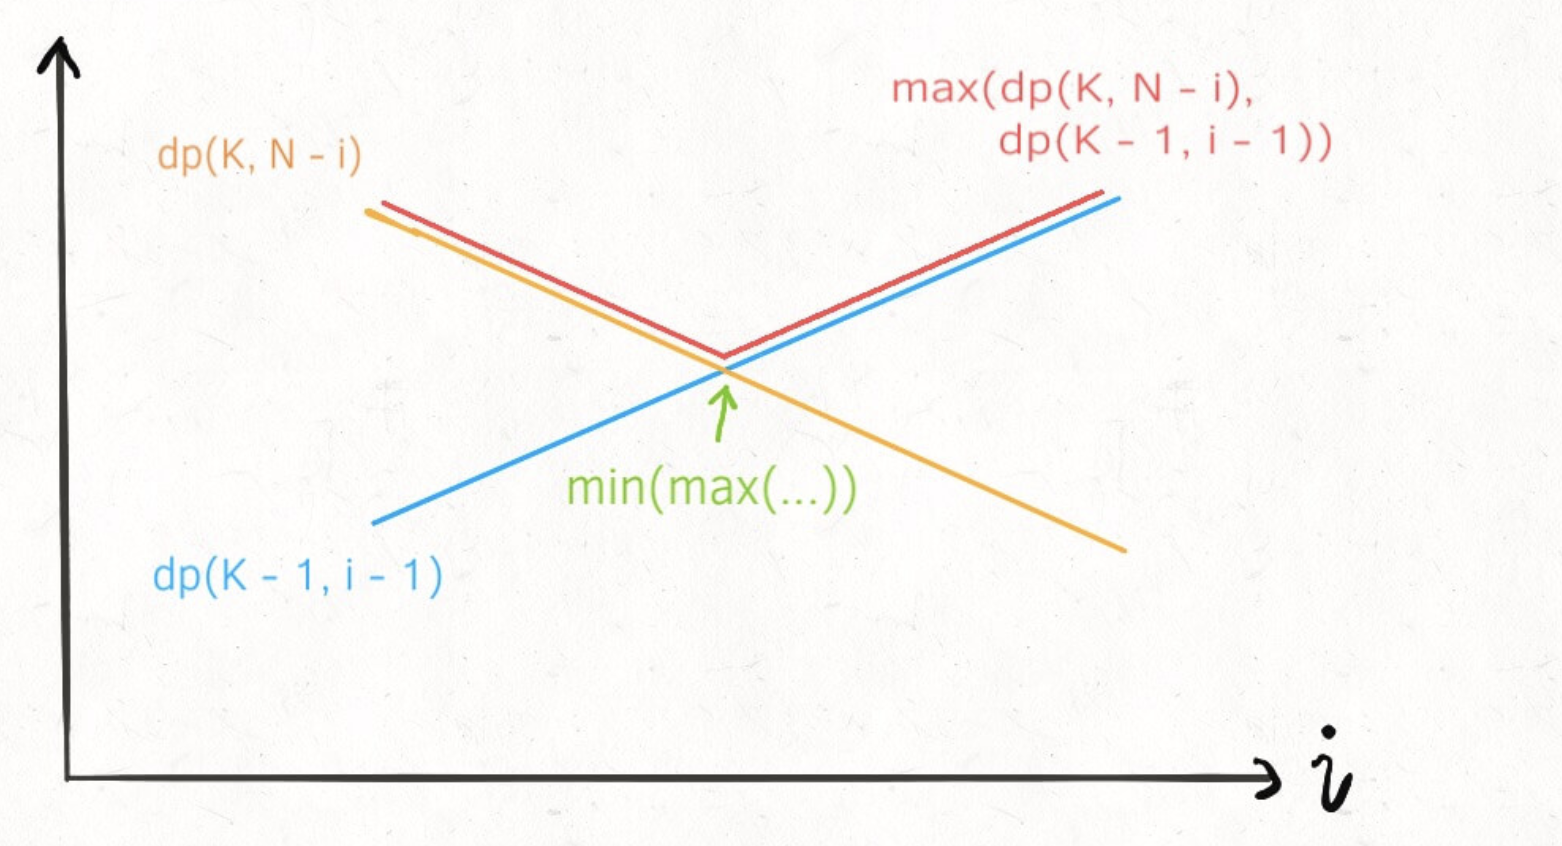
\includegraphics[width=.5\textwidth]{fig/Dynamic_Programming_Egg_Throw_1.png}
\end{figure}

这时候求二者的较大值,再求这些最大值之中的最小值,其实就是求这个交点嘛,熟悉二分搜索的同学肯定敏感地想到了,这不就是相当于求 Valley(山谷)值嘛,可以用二分查找来快速寻找这个点的。直接贴一下代码吧,思路还是完全一样的:
\begin{lstlisting}
def superEggDrop(self, K: int, N: int) -> int:
        
    memo = dict()
    def dp(K, N):
        if K == 1: return N
        if N == 0: return 0
        if (K, N) in memo:
            return memo[(K, N)]
                            
        # for 1 <= i <= N:
        #     res = min(res, 
        #             max( 
    #                     dp(K - 1, i - 1), 
    #                     dp(K, N - i)      
        #                 ) + 1 
        #             )

        res = float('INF')
        # 用二分搜索代替线性搜索
        lo, hi = 1, N
        while lo <= hi:
            mid = (lo + hi) // 2
            broken = dp(K - 1, mid - 1) # 碎
            not_broken = dp(K, N - mid) # 没碎
            # res = min(max(碎,没碎) + 1)
            if broken > not_broken:
                hi = mid - 1
                res = min(res, broken + 1)
            else:
                lo = mid + 1
                res = min(res, not_broken + 1)

        memo[(K, N)] = res
        return res
    
    return dp(K, N)
\end{lstlisting}
这个算法的时间复杂度是多少呢?动态规划算法的时间复杂度就是子问题个数 × 函数本身的复杂度。

函数本身的复杂度就是忽略递归部分的复杂度,这里 dp 函数中用了一个二分搜索,所以函数本身的复杂度是 O(logN)。

子问题个数也就是不同状态组合的总数,显然是两个状态的乘积,也就是 O(KN)。

所以算法的总时间复杂度是 $O(K*N*logN)$, 空间复杂度 O(KN)。效率上比之前的算法 $O(KN^2)$ 要高效一些。

\subsubsection{重新定义状态转移}
前文「不同定义有不同解法」就提过,找动态规划的状态转移本就是见仁见智,比较玄学的事情,不同的状态定义可以衍生出不同的解法,其解法和复杂程度都可能有巨大差异。这里就是一个很好的例子。

再回顾一下我们之前定义的 dp 数组含义:
\begin{lstlisting}
def dp(k, n) -> int
# 当前状态为 k 个鸡蛋,面对 n 层楼
# 返回这个状态下最少的扔鸡蛋次数
\end{lstlisting}

用 dp 数组表示的话也是一样的:
\begin{lstlisting}
dp[k][n] = m
# 当前状态为 k 个鸡蛋,面对 n 层楼
# 这个状态下最少的扔鸡蛋次数为 m
\end{lstlisting}

按照这个定义,就是确定当前的鸡蛋个数和面对的楼层数,就知道最小扔鸡蛋次数。最终我们想要的答案就是 dp(K, N) 的结果。

这种思路下,肯定要穷举所有可能的扔法的,用二分搜索优化也只是做了「剪枝」,减小了搜索空间,但本质思路没有变,还是穷举。

现在,我们稍微修改 dp 数组的定义,确定当前的鸡蛋个数和最多允许的扔鸡蛋次数,就知道能够确定 F 的最高楼层数。具体来说是这个意思:
\begin{lstlisting}
dp[k][m] = n
# 当前有 k 个鸡蛋,可以尝试扔 m 次鸡蛋
# 这个状态下,最坏情况下最多能确切测试一栋 n 层的楼

# 比如说 dp[1][7] = 7 表示:
# 现在有 1 个鸡蛋,允许你扔 7 次;
# 这个状态下最多给你 7 层楼,
# 使得你可以确定楼层 F 使得鸡蛋恰好摔不碎
# (一层一层线性探查嘛)
\end{lstlisting}

这其实就是我们原始思路的一个「反向」版本,我们先不管这种思路的状态转移怎么写,先来思考一下这种定义之下,最终想求的答案是什么?

我们最终要求的其实是扔鸡蛋次数 m,但是这时候 m 在状态之中而不是 dp 数组的结果,可以这样处理:
\begin{lstlisting}
int superEggDrop(int K, int N) {

    int m = 0;
    while (dp[K][m] < N) {
        m++;
        // 状态转移...
    }
    return m;
}
\end{lstlisting}

题目不是给你 K 鸡蛋,N 层楼,让你求最坏情况下最少的测试次数 m 吗?while 循环结束的条件是 dp[K][m] == N,也就是给你 K 个鸡蛋,测试 m 次,最坏情况下最多能测试 N 层楼。

注意看这两段描述,是完全一样的!所以说这样组织代码是正确的,关键就是状态转移方程怎么找呢?还得从我们原始的思路开始讲。之前的解法配了这样图帮助大家理解状态转移思路:
\begin{figure}[H]
    \centering
    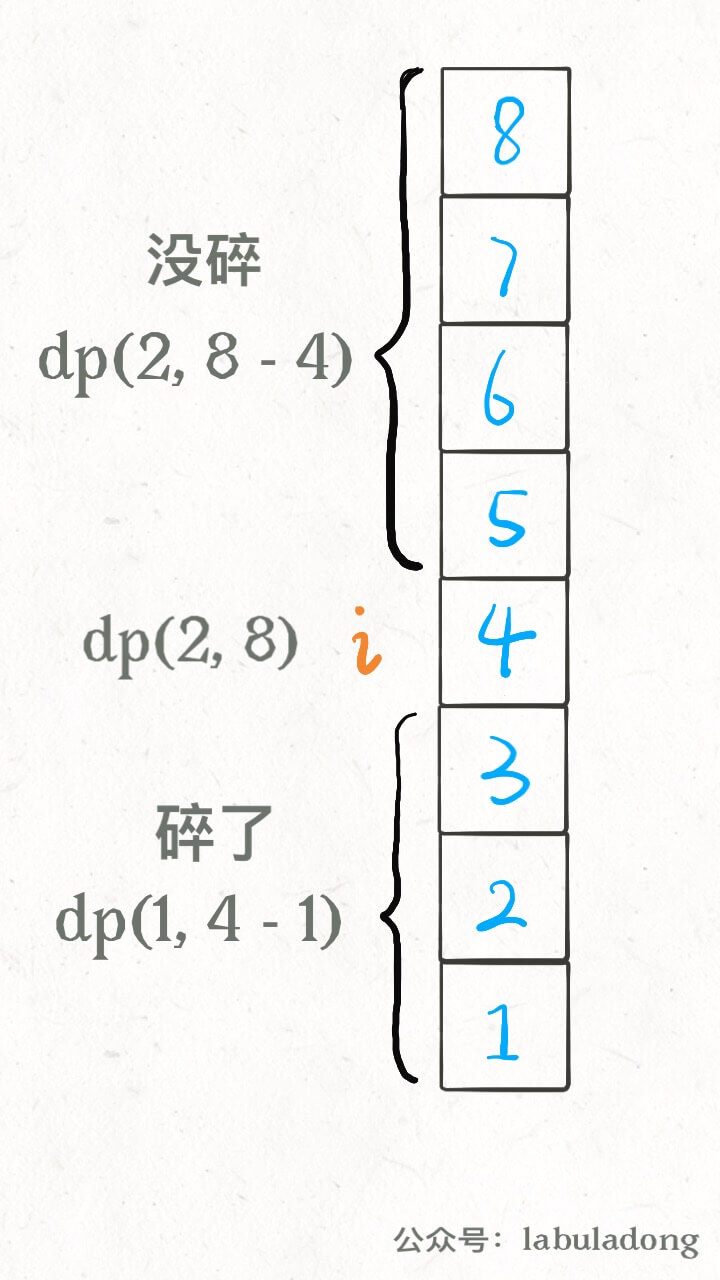
\includegraphics[width=.4\textwidth]{fig/Dynamic_Programming_Egg_Throw_2.jpg}
\end{figure}

这个图描述的仅仅是某一个楼层 i,原始解法还得线性或者二分扫描所有楼层,要求最大值、最小值。但是现在这种 dp 定义根本不需要这些了,基于下面两个事实:

1、无论你在哪层楼扔鸡蛋,鸡蛋只可能摔碎或者没摔碎,碎了的话就测楼下,没碎的话就测楼上。

2、无论你上楼还是下楼,总的楼层数 = 楼上的楼层数 + 楼下的楼层数 + 1(当前这层楼)。

根据这个特点,可以写出下面的状态转移方程:

dp[k][m] = dp[k][m - 1] + dp[k - 1][m - 1] + 1

dp[k][m - 1] 就是楼上的楼层数,因为鸡蛋个数 k 不变,也就是鸡蛋没碎,扔鸡蛋次数 m 减一;dp[k - 1][m - 1] 就是楼下的楼层数,因为鸡蛋个数 k 减一,也就是鸡蛋碎了,同时扔鸡蛋次数 m 减一。PS:这个 m 为什么要减一而不是加一?之前定义得很清楚,这个 m 是一个允许的次数上界,而不是扔了几次。
\begin{figure}[H]
    \centering
    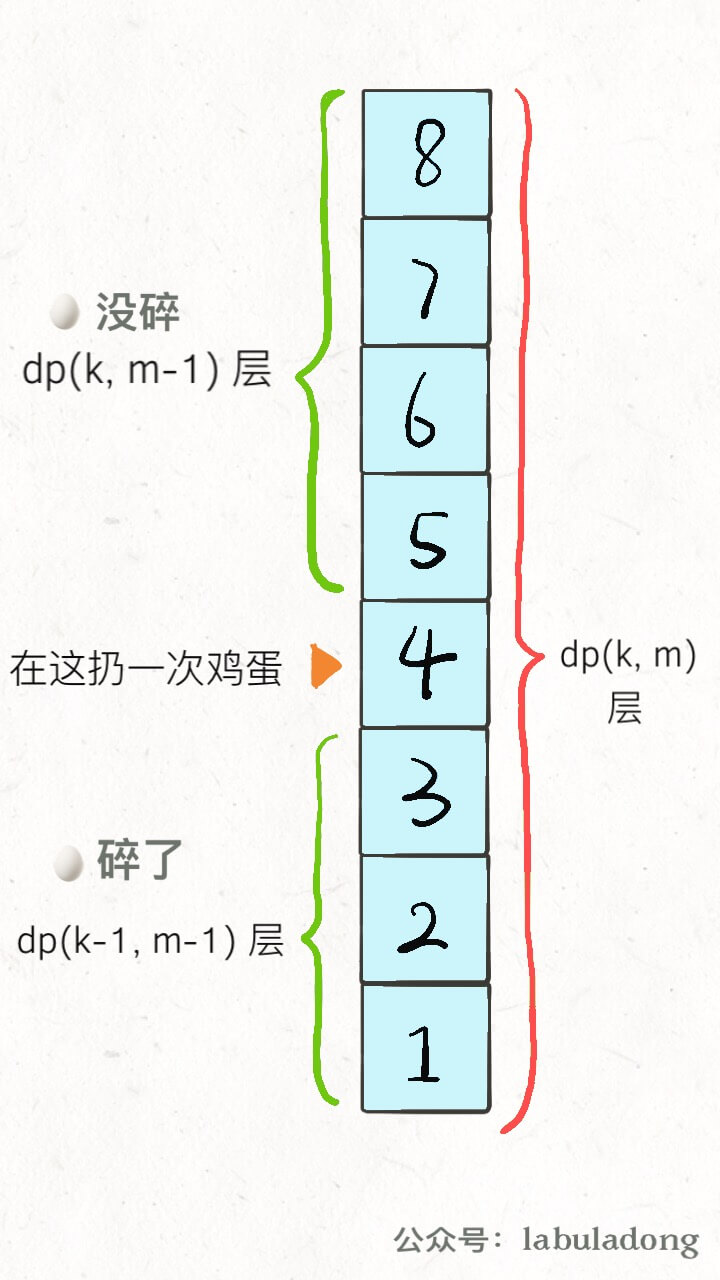
\includegraphics[width=.4\textwidth]{fig/Dynamic_Programming_Egg_Throw_3.jpg}
\end{figure}

至此,整个思路就完成了,只要把状态转移方程填进框架即可:
\begin{lstlisting}
int superEggDrop(int K, int N) {
    // m 最多不会超过 N 次(线性扫描)
    int[][] dp = new int[K + 1][N + 1];
    // base case:
    // dp[0][..] = 0
    // dp[..][0] = 0
    // Java 默认初始化数组都为 0
    int m = 0;
    while (dp[K][m] < N) {
        m++;
        for (int k = 1; k <= K; k++)
            dp[k][m] = dp[k][m - 1] + dp[k - 1][m - 1] + 1;
    }
    return m;
}
\end{lstlisting}

如果你还觉得这段代码有点难以理解,其实它就等同于这样写:
\begin{lstlisting}
for (int m = 1; dp[K][m] < N; m++)
    for (int k = 1; k <= K; k++)
        dp[k][m] = dp[k][m - 1] + dp[k - 1][m - 1] + 1;
\end{lstlisting}

看到这种代码形式就熟悉多了吧,因为我们要求的不是 dp 数组里的值,而是某个符合条件的索引 m,所以用 while 循环来找到这个 m 而已。

这个算法的时间复杂度是多少?很明显就是两个嵌套循环的复杂度 O(KN)。

另外注意到 dp[m][k] 转移只和左边和左上的两个状态有关,所以很容易优化成一维 dp 数组,这里就不写了。

\subsubsection{还可以再优化}
再往下就要用一些数学方法了,不具体展开,就简单提一下思路吧。在刚才的思路之上,注意函数 dp(m, k) 是随着 m 单增的,因为鸡蛋个数 k 不变时,允许的测试次数越多,可测试的楼层就越高。

这里又可以借助二分搜索算法快速逼近 dp[K][m] == N 这个终止条件,时间复杂度进一步下降为 O(KlogN),我们可以设 g(k, m) =……

算了算了,打住吧。我觉得我们能够写出 O(K*N*logN) 的二分优化算法就行了,后面的这些解法呢,听个响鼓个掌就行了,把欲望限制在能力的范围之内才能拥有快乐!

不过可以肯定的是,根据二分搜索代替线性扫描 m 的取值,代码的大致框架肯定是修改穷举 m 的 for 循环:
\begin{lstlisting}
// 把线性搜索改成二分搜索
// for (int m = 1; dp[K][m] < N; m++)
int lo = 1, hi = N;
while (lo < hi) {
    int mid = (lo + hi) / 2;
    if (... < N) {
        lo = ...
    } else {
        hi = ...
    }
    
    for (int k = 1; k <= K; k++)
        // 状态转移方程
}
\end{lstlisting}

\section{动态规划之子序列问题解题模板}
子序列问题是常见的算法问题,而且并不好解决。

首先,子序列问题本身就相对子串、子数组更困难一些,因为前者是不连续的序列,而后两者是连续的,就算穷举你都不一定会,更别说求解相关的算法问题了。

而且,子序列问题很可能涉及到两个字符串,比如「最长公共子序列」,如果没有一定的处理经验,真的不容易想出来。所以本文就来扒一扒子序列问题的套路,其实就有两种模板,相关问题只要往这两种思路上想,十拿九稳。

一般来说,这类问题都是让你求一个最长子序列,因为最短子序列就是一个字符嘛,没啥可问的。一旦涉及到子序列和最值,那几乎可以肯定,考察的是动态规划技巧,时间复杂度一般都是 $O(n^2)$。

原因很简单,你想想一个字符串,它的子序列有多少种可能?起码是指数级的吧,这种情况下,不用动态规划技巧,还想怎么着?

既然要用动态规划,那就要定义 dp 数组,找状态转移关系。我们说的两种思路模板,就是 dp 数组的定义思路。不同的问题可能需要不同的 dp 数组定义来解决。

\subsection{两种思路}
第一种思路模板是一个一维的 dp 数组:
\begin{lstlisting}
int n = array.length;
int[] dp = new int[n];

for (int i = 1; i < n; i++) {
    for (int j = 0; j < i; j++) {
        dp[i] = 最值(dp[i], dp[j] + ...)
    }
}
\end{lstlisting}

比如对于「最长递增子序列」,在这个思路中 dp 数组的定义是:在子数组 array[0..i] 中,我们要求的子序列(最长递增子序列)的长度是 dp[i]。为啥最长递增子序列需要这种思路呢?前文说得很清楚了,因为这样符合归纳法,可以找到状态转移的关系,这里就不具体展开了。

第二种思路模板是一个二维的 dp 数组:
\begin{lstlisting}
int n = arr.length;
int[][] dp = new int[n][n];

for (int i = 0; i < n; i++) {
    for (int j = 0; j < n; j++) {
        if (arr[i] == arr[j]) 
            dp[i][j] = dp[i][j] + ...
        else
            dp[i][j] = 最值(...)
    }
}
\end{lstlisting}
这种思路运用相对更多一些,尤其是涉及两个字符串/数组的子序列,比如「最长公共子序列」。本思路中 dp 数组含义又分为「只涉及一个字符串」和「涉及两个字符串」两种情况:
\begin{itemize}
\setlength{\itemsep}{0pt}
\setlength{\parsep}{0pt}
\setlength{\parskip}{0pt}
    \item 涉及两个字符串/数组时(比如最长公共子序列),dp 数组的含义如下:在子数组 arr1[0..i] 和子数组 arr2[0..j] 中,我们要求的子序列(最长公共子序列)长度为 dp[i][j]。参见「编辑距离」、「公共子序列」;
    \item 只涉及一个字符串/数组时(比如本文要讲的最长回文子序列),dp 数组的含义如下:在子数组 array[i..j] 中,我们要求的子序列(最长回文子序列)的长度为 dp[i][j]。参见如下的最长回文子序列。
\end{itemize}

\subsection{最长回文子序列}



\section{最后总结}
\textbf{计算机解决问题其实没有任何奇技淫巧,它唯一的解决办法就是穷举,穷举所有可能性}。算法设计无非就是先思考“如何穷举”,然后再追求“如何聪明地穷举”。

列出动态转移方程,就是在解决“如何穷举”的问题。之所以说它难,一是因为很多穷举需要递归实现,二是因为有的问题本身的解空间复杂,不那么容易穷举完整。

备忘录、DP table 就是在追求“如何聪明地穷举”。用空间换时间的思路,是降低时间复杂度的不二法门。

%\printbibliography
\bibliography{../ref}
\bibliographystyle{IEEEtran}
\end{document}
